\documentclass[a4paper]{report}

\usepackage[masterthesis,english]{comp}
\usepackage{graphicx}
\usepackage{hyperref}
\usepackage{multirow}
\usepackage{mathtools}
\usepackage{listings}
\usepackage{color}
\usepackage{multicol}
\usepackage{wrapfig}

\definecolor{mygreen}{rgb}{0,0.6,0}
\definecolor{mygray}{rgb}{0.5,0.5,0.5}
\definecolor{mymauve}{rgb}{0.58,0,0.82}

\lstset{ %
  backgroundcolor=\color{white},   % choose the background color; you must add \usepackage{color} or \usepackage{xcolor}
  basicstyle=\footnotesize,        % the size of the fonts that are used for the code
  breakatwhitespace=false,         % sets if automatic breaks should only happen at whitespace
  breaklines=true,                 % sets automatic line breaking
  captionpos=b,                    % sets the caption-position to bottom
  commentstyle=\color{mygreen},    % comment style
  extendedchars=true,              % lets you use non-ASCII characters; for 8-bits encodings only, does not work with UTF-8
  keepspaces=true,                 % keeps spaces in text, useful for keeping indentation of code (possibly needs columns=flexible)
  keywordstyle=\color{blue},       % keyword style
  numbers=left,                    % where to put the line-numbers; possible values are (none, left, right)
  numbersep=5pt,                   % how far the line-numbers are from the code
  numberstyle=\tiny\color{mygray}, % the style that is used for the line-numbers
  rulecolor=\color{black},         % if not set, the frame-color may be changed on line-breaks within not-black text (e.g. comments (green here))
  showspaces=false,                % show spaces everywhere adding particular underscores; it overrides 'showstringspaces'
  showstringspaces=false,          % underline spaces within strings only
  showtabs=false,                  % show tabs within strings adding particular underscores
  stringstyle=\color{mymauve},     % string literal style
  tabsize=2,                       % sets default tabsize to 2 spaces
  title=\lstname
}

\title{A General Framework For Aspect Oriented Programming}
\author{Chris Vesters}
\principaladviser{Dirk Janssens}
\assistantadviser{Tim Molderez}
\submitdate{June 2014}
\bibpunct{[}{]}{;}{a}{,}{,}
\bibfile{references}

% Make hyperref package use black links
\hypersetup{
	pdfauthor={Chris Vesters},
	pdftitle={A General Framework For Aspect Oriented Programming},
	pdfkeywords={Aspect Oriented Programming, Framework},
    colorlinks,
    citecolor=black,
    filecolor=black,
    linkcolor=black,
    urlcolor=black
}

\begin{document}
\frontpages

\clearpage 
\phantomsection 
\addcontentsline{toc}{chapter}{Nederlandstalige Samenvatting}
\chapter*{Nederlandstalige Samenvatting}
Aspect oriented programming languages worden momenteel vaak gebaseerd op een bestaande taal, waaraan dergelijke elementen worden toegevoegd. Deze extensie is vrij verregaand en vergt behoorlijk wat werk doordat ze altijd vanaf nul moet worden begonnen. Bovendien merken we op dat in de uiteindelijke taal vaak de basistaal en aspect oriented langauge gemengd zijn, waardoor hergebruik van de aspect elementen onmogelijk wordt.\\
\\
In deze thesis stellen we een framework voor dat de kernelementen van aspect oriented programming bevat volledig los van elke basistaal. De bedoeling van dit framework is om het mogelijk te maken om nieuwe en reeds bestaande talen te voorzien met aspect oriented programming. De grootste uitdaging is het vinden van een balans tussen de abstractie en het vereiste werk. Een framework dat niet abstract genoeg is, zal slechts in enkele gevallen bruikbaar zijn, terwijl een te abstract framework geen bijdrage levert tot het verminderen van het benodigde wrerk.\\
\\
De capaciteiten en gebreken worden aangetoond door middel van Small C en Dot te voorzien van aspect oriented programming. Omdat het op korte termijn onmoglijk is om voor meerdere verschillende talen het framework te testen, is gekozen om voor andere aspect oriented talen na te gaan hoe deze door gebruik te maken van het framework geimplementeerd zouden kunnen worden.\\
\\
De resultaten zijn afhankelijk van de beschikbare tools en de gewenste features, maar algemeen kan gesteld worden dat het framework in staat is om verschillende soorten talen te ondersteunen en dit veel sneller dan bij het beginnen vanaf nul.

\clearpage 
\phantomsection 
\addcontentsline{toc}{chapter}{Acknowledgements}
\chapter*{Acknowledgements}
I would like to thank Tim Molderez for guiding me during the entire process and professor Janssens for making this thesis possible. I would also like to thank my family and friends for supporting me during the entire period, and pulling me through all the work. Lastly I would like to thank the creators of ANTLR and ObjectAid for the creation of this software which made my work a lot easier.
\clearpage 
\phantomsection 
\addcontentsline{toc}{chapter}{Abstract}
\chapter*{Abstract}
Aspect oriented programming languages are often based on an existing base language to which aspect oriented elements are added. This extension is pretty invasive and takes a lot of work since it is done from scratch. We also not that the resulting language is mixed with the base language, making re-use of the aspect elements impossible.\\
\\
A framework is presented that contains all core elements of aspect oriented programming and is completely independent of any base language. The goal is to make it possible to extend the framework and provide new and existing languages with aspect oriented programming. The biggest challenge is the trade-off between the level of abstraction and the work required to extend it. A framework that does not sufficiently abstract from the base language can only be used for certain languages, while to much abstraction wouldn't add any value as the amount of work to extend it would be the same a starting from scratch.\\
\\
We show the functionality of the framework by using it on Small C and Dot. For other aspect oriented languages we examine how the same features could be provided by the framework.

\mainbodypages

\chapter{Introduction}
\section{Aspect Oriented Programming}
Aspect oriented programming (from now on referred to as AOP) is a way of programming that allows separating code beyond the capabilities of object oriented programming. It allows the separation of cross cutting concerns from the core concerns, by doing this we achieve more modular code, prevent code tangling and code scattering which results in code that is easier to maintain and modify.
\begin{figure}[h!]
\centering
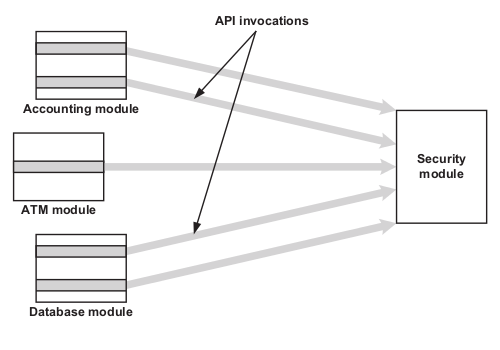
\includegraphics[scale=0.5]{images/Code_Scattering.png}
\caption{A representation of code scattering\cite{Laddad10}.}
\label{fig:Code_Scattering}
\end{figure}\\
\begin{figure}[h!]
\centering
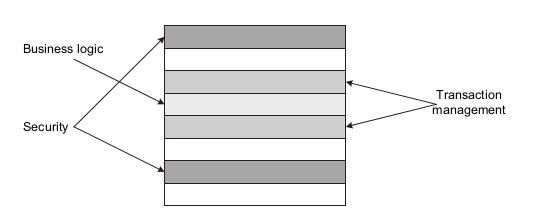
\includegraphics[scale=0.5]{images/Code_Tangling.png}
\caption{A representation of code tangling\cite{Laddad10}.}
\label{fig:Code_Tangling}
\end{figure}\\
AOP works by identifying join points, which is certain point in the execution of the program. The set of all the join points is called the join point model. It is at these join points that we can modify the original program execution. This change can go from something as simple as logging to something more invasive where the original code isn't even executed at all.\\
A first thing we need is a way to indicate which join points we want to work on, this is done by a point cut. Now we can refer to certain join points we also need a way to modify the execution. This is done by an advice, note that there can be multiple kinds of advice.\\
In the end everything has to come together, this is done by the weaver.\\
\\
The most known AOP language by far is AspectJ, which is an extension of Java. To demonstrate the concept of AOP a couple of AspectJ examples are shown here:\\
TODO: EXAMPLES!\\

\section{Problem}
Currently AOP is often implemented by extending an existing language, this often leads to completely new languages requiring new compilers and  breaking existing tools for the base language. Especially the latter is a reason why some people haven't made the step to start working with aspect oriented languages.\\
\\
Though the concepts of AOP are quite general, which is reflected by the similarities in different aspect oriented languages, all the AOP parts of these languages were written from scratch. The main reason for this is the absence of a general language independent library or framework to handle aspect orientation. Another reasons is that by building a language from scratch you get more freedom to implement the desired features.

\section{Goal}
The goal of this thesis is to build a framework that encloses all core ideas of AOP in an abstract manner without being specific about a particular base language. This will enable use to use the framework to develop an aspect oriented language quicker and easier than currently is the case by extending a couple of parts. The framework will work for completely new languages, and existing ones we want to extend. The latter one will pose the most problems as the freedom to adapt the compiler is very limited.

\chapter{Aspect Oriented Language Components}
An aspect oriented language consists of several components, to explain these I will start from the base language and work my way up to get an aspect oriented language. At every point I'll make it more concrete with a small AspectJ example.\\
\\
The starting point of creating an aspect oriented language is the base language, this is the language that we want to extend or is a completely new language. In the latter case the base language will be the new language excluding all the aspect oriented features. The base language can be any kind of language: procedural, object oriented, functional, logical, data oriented, ...\\
\\
By defining the base language we implicitly defined a join point model. This is because the join point model consists of all the points that occur during execution on which intervention of the aspects is allowed. The join point model will always remain implicit, but it is an important part of any aspect oriented language as it is the link between the base language and the aspect oriented part.\\
\\
Knowing at which points we can intervene doesn't allow us to do anything, we need a way to identify certain points. This identification is done by using pointcuts, specifying one or more join points. They way in which pointcuts allow us to refer to join points should be as close as possible as the way in which they appear in the base language. If we look at an example of AspectJ (TODO: ADD), we clearly see the similarities.
\\
Now that we can refer to certain join points, we can actually start modifying the original code. This modification is encapsulated in an advice, which contains 'code' that has to be executed. When this 'code' is executed is defined by the pointcut with which the advice is associated. Whenever the program passes a join point that matches with the associated pointcut, this advice must be executed. The 'code' in the advice should be written in the base language to prevent the user from learning an entire new language. (TODO: EXAMPLE) The advice should also be able to have access to information about the join point, this information will be provided by the pointcut.\\
\\
One problem that arises is: what is suppose to happen if we encounter a join point at which multiple advices are to be executed? This can be either caused by multiple pointcuts matching to the join point, or multiple advices being associated with the same pointcut. The latter case can be easily solved as we can combine the two advices into one bigger advice. The first is a bit more tricky since the one pointcut can also match other join points, different from the other, which means we can't just combine them. (TODO: illustrate) The solution to this is of course to introduce an ordering mechanism. This ordering can be either placed on the pointcuts or on the advices, in the first case we still need to make sure that there is only one advice for each pointcut though.\\
\\
One final component we need, is something that will actually make sure that the advices are executed when the join points are encountered. The weaver will make this happen, and can do this in multiple ways. The easiest is compile-time, weaving which comes down to a pre-processing step, a more advanced form is run-time weaving, yet other forms are available depending on the base language. (TODO: EXAMPLE)\\
\\
With the components specified above we are perfectly possible to create an aspect oriented language, despite that we note that some features are still missing, as an example we note that communication between different advices is impossible. Since aspect orientation is often presented as an extension of object oriented programming it makes sense to introduce some form of class, called aspects. These aspects will contain the advices, which match functions and methods in object oriented languages, and can be extended to have members too. By doing this we immediately have can provide the advantages offered by object oriented languages among which are inheritance and encapsulation. (TODO: EXAMPLE)\\
\\
An overview of all the components and how they are linked together is shown in figure (TODO:REF). The weaver is not considered to be part of the aspect language just as a compiler is not considered a part of the language.

\chapter{Aspect Oriented Framework}
Since the framework has the be easily extensible to work with any kind of language it has to be very abstract and may not contain any information about a base language. On the other hand, creating a framework that is too abstract and general requires too many additions to be made to implement it for a base language, making the framework completely missing its goal. The level of abstraction has to be well considered.\\
\\
I will first go into detail how the components that were identified in the previous chapter are represented and work in the framework. The explanation of the weaver is preceded by some information that is required to fully understand how the weaver works. This is followed by some remarks about the current version of the framework, and to conclude the chapter I explain how we can now expand this framework to work with any base language.\\
\\
The first component of the aspect language that we identified were the pointcuts. This component is implemented as an abstract class Pointcut, to completely specify a join point we need some way to identify it's signature, this however is language specific and can therefore not be provided by the framework. Other common structures are arguments and context. The arguments are meant for information that can be used in the advice, while the context is a way to restrict matching join points based on  information that goes beyond the scope of the join point.\\
\\
Something we notice, which is also the case for AspectJ, is that it is not possible to identify completely different join points with one pointcut. This complicates writing advice that has to be executed on these two different sets of join points. To simplify this we allow grouping pointcuts into sets, implemented as a PointcutSet as can be seen in figure \ref{fig:PointcutSet}, which has a set of pointcuts. Arguments that are available for the advice should be present in all the poincuts of the set and they should match names so we can link them from advice to this pointcut.
\begin{figure}[h!]
\centering
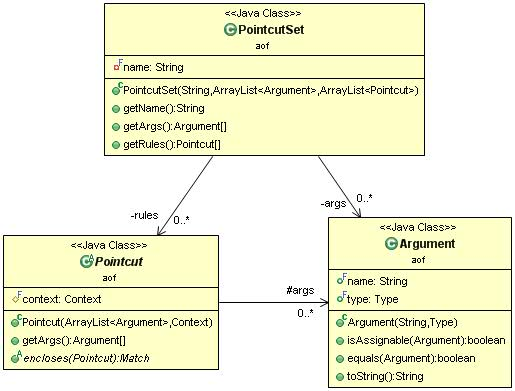
\includegraphics[scale=0.7]{images/AOF/PointcutSet.jpg}
\caption{UML diagram of the PointcutSet and Pointcut.}
\label{fig:PointcutSet}
\end{figure}\\
\\
The advices are implemented by the abstract Advice class. This class has a name, which will make ordering them a lot easier, and a set of arguments, these arguments are the ones that can be used inside the advice body. Note that the arguments of the pointcut to which this advice is linked must be assignable to these arguments. The body or actual code of the advice is not provided by this class, simply because it depends on the base language as we want this to be in the same formalism. The UML diagram of the class is shown in figure \ref{fig:Advice}.
\begin{figure}[h!]
\centering
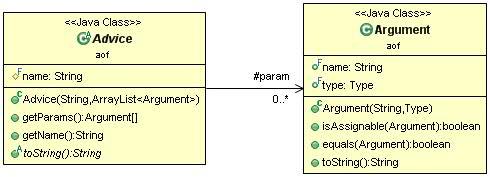
\includegraphics[scale=0.7]{images/AOF/Advice.jpg}
\caption{UML diagram of the Advice.}
\label{fig:Advice}
\end{figure}\\
\\
Before going any further some more explanation about some already mentioned concepts is required. I have talked about arguments and a context, but didn't mention what these are. An argument is a hard to abstract as every base language has its own vision of what an argument is, though two concepts are very common, being a name and a type. For this reason the Argument class has a name, which is also required for access to the argument and a type. The type however can not be a base language type, but should be more general. For this reason an interface called Type was created. A context is easier, since  the context can be anything and highly depends on the base language the only thing the framework provides is an interface Context. Note that the Context and Type interface are exactly the same, I will discuss this into more detail in chapter \ref{chap:Discussion}.
\begin{figure}[h!]
\centering
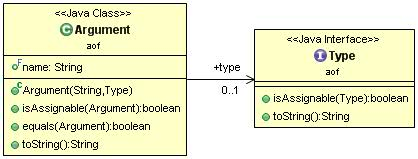
\includegraphics[scale=0.7]{images/AOF/Argument.jpg}
\caption{UML diagram of the Argument class.}
\label{fig:Argument}
\end{figure}\\
\begin{figure}[h!]
\centering
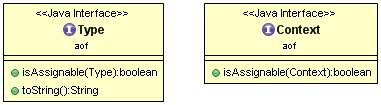
\includegraphics[scale=0.7]{images/AOF/Type-Context.jpg}
\caption{UML diagram of the Type and Context interface.}
\label{fig:Type-Context}
\end{figure}\\
\\
This being said we can now discuss the remaining components being: the order mechanism, the aspect and the weaver. The components will be handled in the order they are specified here.\\
\\
The framework does not provide a basis for the ordering. This means that the user is free to implement the way of specifying an ordering as he likes. The user is also free to choose whether the order will be specified on the pointcuts or on the advice. Despite the freedom on the ordering 'language' the ordering itself is still limited. This will be discussed into more detail once the weaver is introduced.\\
\\
The current version of the framework does not provide any concept of 'aspects', though this causes some limitations, it does not make the framework useless. Some of the limitations were already mentioned in the previous chapter, more details about the consequences of the absence of an encapsulating aspect is discussed at the end of this chapter.\\
\\
Before discussing the weaver we have to make some things a bit clearer. You might be wondering how the join points will be extracted from the source code. This is done by the parser of the base language, or a modification of it. The join points that are generated by this parser will actually be instances of the Pointcut class. By doing this comparing whether a pointcut set contains a pointcut that matches the joinpoint becomes trivial.\\
\\
Something you might have noticed is that the advice does not keep a link to the pointcut itself, nor the other way around. The link between pointcut and advices is handled by the weaver, this allows a better separation between pointcuts and advices and gives the weaver more freedom to operate.\\
\\
The ordering mechanism requires some extra information as well, I mentioned earlier that despite the freedom some limitations still exist. This is cause by the way the weaver handles the ordering internally. The weaver will keep a list for every advice to its preceding advices. This means that the ordering provided to the weaver has to be on the advices, and should result in a partial ordering. To clarify things a small example is given. The partial ordering shown in figure \ref{fig:Order} can result into several orders among which:
\begin{itemize}
\item A; B; C; D; E; F; G
\item A; C; B; D; E; F; G
\item A; D; C; B; E; F; G
\item A; D; C; E; G; B; F
\end{itemize}
Which order is chosen is unpredictable, and it shouldn't matter as no order was specified among those elements.\\
\begin{figure}[h!]
\centering
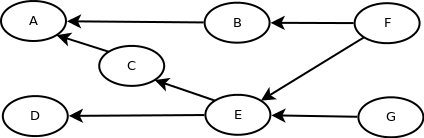
\includegraphics[scale=0.6]{images/AOF/Order.png}
\caption{A partial ordering of seven advices.}
\label{fig:Order}
\end{figure}\\
A final remark that has to be made is how the framework handles the argument mapping from adivce to pointcut and join point. For this the framework provides a Match class, shown in figure \ref{fig:Match}, that contains a dynamic value for each argument. We can use this match to get the join point specific value for an argument of the advice.
\begin{figure}[h!]
\centering
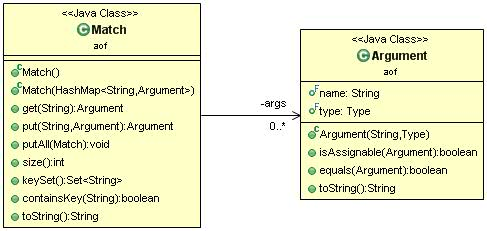
\includegraphics[scale=0.7]{images/AOF/Match.jpg}
\caption{UML diagram of the Match class.}
\label{fig:Match}
\end{figure}\\
\\
This brings us to the last component, the weaver. Just like most elements in the framework is the weaver implemented as an abstract class. This abstract class provides a way for all components to register their information, which is then stored to be processed. How this information can be processed or the preferred way to do it, depends on the base language and the possibilities of its parser, and can therefor not be implemented by the framework. The framework does however provide a way to specify the input and output files by using flags, which are shown in \ref{tab:Flags}.\\
\begin{table}[h]
\centering
\begin{tabular}{l l}
-a \textit{files} & Specify the aspect files.\\ [2ex]
-s \textit{files} & Specify the source files.\\ [2ex]
-oDir \textit{dir} & Specify an output directory (optionally).\\
\end{tabular}
\caption{An overview of the flags available in the weaver.}
\label{tab:Flags}
\end{table}\\
Besides that it also provides some methods that simplify processing the information. The most important one is 'executingAdvices', given a certain joinpoint this method will return all the advices that have to be executed in the order they are returned. In case the user needs to know the pointcuts that match a certain joinpoint a method 'enclosingPointcuts' is provided. The framework also implements a way to compare advices based on the partial ordering, this is done by the AdviceComparator which is an extension of the Comparator. This is meant for internal usage and the user should not need to use this since the return value of the 'executingAdvices' method is already ordered. A complete overview of the API is shown in figure \ref{fig:Weaver}
\begin{figure}[h!]
\centering
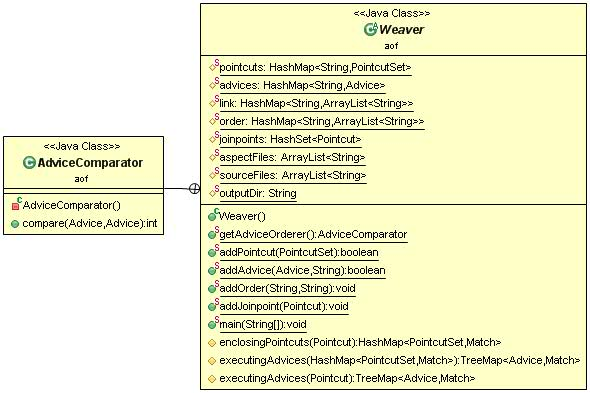
\includegraphics[scale=0.7]{images/AOF/Weaver.jpg}
\caption{UML diagram of the Weaver class.}
\label{fig:Weaver}
\end{figure}\\
\\
A complete overview of the framework and how everything is connected can be seen in figure \ref{fig:FullView}.
\begin{figure}
\centering
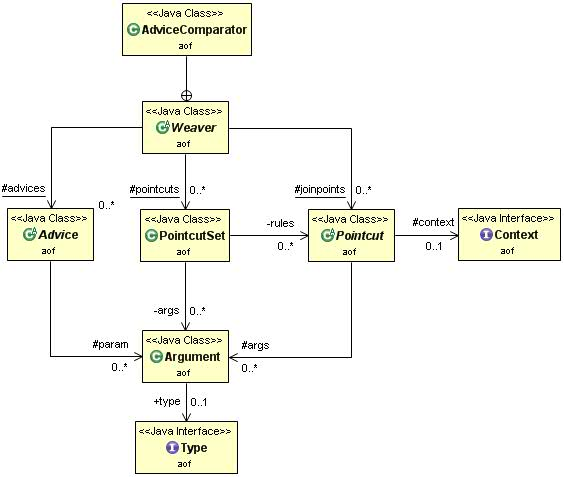
\includegraphics[scale=0.65]{images/AOF/Full.jpg}
\caption{UML diagram of the entire framework.}
\label{fig:FullView}
\end{figure}
Some trade offs had to be made when designing the framework, which I will now discuss into more detail.\\
\\
First of all it needs to be noted that both Context and Type are interfaces which both specify only one method called 'isAssignable'. This means that Context and Type, though called different, do the same thing. We could use one general interface, this is not done though to be able to handle future evolution.\\
\\
Adding a notion of aspect would allow a lot of nice features such as adding members that can be used for communication between advice and inheritance. They could also be used as a way to encapsulate pointcuts and advice, though this can also be done without aspects simply by separating them over multiple files. Adding aspects to the framework would have introduced a lot of extra complexity. Since the goal of this thesis is to demonstrate the usability of such a framework I have chosen to not include this, but keep it as a future work.\\
\\
The framework uses an abstract notion of type, this is to achieve the level abstraction required to separate the framework from the base language. This however means that for each base language we need a new type system that implements the Type interface, which might result in a lot of work. Sometimes it is however possible to use the same type system the compiler of the base language uses if we can add the interface to it.\\
\\
The advice and pointcuts are not directly connected with each other, the connection is achieved by the weaver. Because adding an explicit link does not provide any advantages, I have chosen to do it this way to ensure that the components are as loosely coupled as possible. Nevertheless the framework demands that at the moment a pointcut is added the pointcut set it is linked with must be be known to the compiler.\\
\\
Something that was not discussed so far is what happens if a join point is encountered that is matched by multiple pointcuts in the same pointcut set. In this case there basically are two options: either we execute the advices for each matched pointcut, or we only select the first matched pointcut of the set. Currently the latter is implemented in the framework, mostly because if we still want the first to happen, we can simply split the pointcut set.\\
\\
One final remark that has to be made is that implementing both join points and poincuts as the same Class can be dangerous since they are not the same. One example is that poincuts can contain wildcards wile join points should not. It may also be feasible to allow specifying types and sub-types in pointcuts, where in the join point the types are fixed and known. This means that we have to use the Poincut class carefully if we use it with a join point.\\
\\
To conclude this chapter I will briefly explain how the framework can be expanded to work with a base language, for more detailed examples I refer to chapters \ref{chap:SmallC} and \ref{chap:Dot} where the framework is expanded for two different languages. Before being able to use the framework you have to specify a language in which it is possible to specify pointcuts, advice and optionally an order. You have to provide a parser for this language, which will create the pointcuts and advices which are handed over to the weaver. Due to the separation of the components it is possible to have separate languages for the pointcuts, advice and order, each with its own parser. In practice this will not be such an attractive option though since it involves a lot of extra work.\\
\\
The pointcuts and advice that has to be created has to be specific for the base language, this means that you first have to create a subclass of Advice and one or more subclasses for Pointcut.
The advice subclass is simple, it must contain the body of the advice. The pointcuts need to contain all information to identify a join point. Since there will be multiple types of pointcuts you will have to implement one subclass for each type of pointcut. If you desire to add a context to the pointcut, you still have to create a class with the Context interface that contains all the context information you want to use.\\
\\
The pointcuts and advices of course require you to implement a type system. Depending on the availability of the type system used by the base language, and more precise the compiler, it is possible to add small modifications to get the type system without much work. If not, this might be a bigger problem.\\
\\
Now you can create pointcuts and advice you still need to expand the Weaver class to add the actual weaving. Since the framework gives you the advices to execute for each join point all the extended weaver has to do is execute these advices at those times. This sounds easier than it sometimes is, especially how you can interact with the base language is important. Eventually it all comes down to putting all the information in the weaver and generating the weaved code. A schematic overview of this is shown in figure \ref{fig:Weaving}, note that the aspect language is split up into three components. It is possible to have this explicit separation, but most of the time this will cause more work to implement and thus not be this explicit.
\begin{figure}
\centering
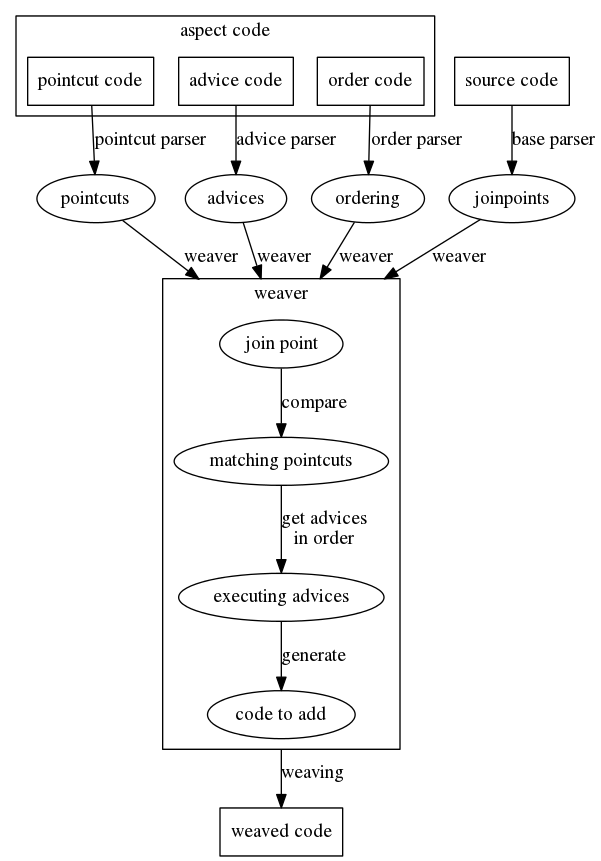
\includegraphics[scale=0.5]{images/AOF/weaving.png}
\caption{Schematic overview of the weaving process}
\label{fig:Weaving}
\end{figure}

\chapter{Small C}
\label{chap:SmallC}
Small C is a subset of the C language, which makes it an procedural language. Though it does not support structs or including other files, it does give us a good overview of what aspect orientation in a procedural programming language is like. Besides this, the presences of a modifiable compiler made this language an interesting first step to test the framework.\\
\\
Despite the resemblance with C, I specify an example, listing \ref{lst:SmallC_Example}, to show the normal structure of a Small C program. This example will also be used later to demonstrate the functionality of the framework.

\begin{lstlisting}[language=C, multicols=2, caption=A simple Small C program., label=lst:SmallC_Example]
#include <stdio.h>

int count = 0;

int mySquare(int a) {
	return a * a;
}

int mySqrt(int a) {
	int i = 1;
	while (mySquare(i) <= a) {
		i = i + 1;
	}	
	return i - 1;
}

void main () {
	int a = 2;
	int b = 10;
	
	x = mySquare(a);
	count = count + 1;
	x = mySqrt(a);
	count = count + 1;
	x = mySqrt(25);
	count = count + 1;
	x = mySquare(count);
	count = count + 1;
}
\end{lstlisting}

\section{Join Point Model}
Due to the minimalistic character of the language the join point model is limited too. The join points identified can be divided into two groups, each with two types. An overview of the join points is given in table \ref{tab:SmallC_JoinPoints}.
\begin{table}
\centering
\begin{tabular}{|l|l|l|}
\hline
Join Point & Type & Description\\
\hline
\multirow{2}{*}{Function} & Call & The moment a function is called.\\
& Execution & The moment a function is executed\\
\hline
\multirow{2}{*}{Global Variable} & Set & The moment a global variable is set.\\
& Get & The moment a global variable is accessed.\\
\hline
\end{tabular}
\caption{Small C join points.}
\label{tab:SmallC_JoinPoints}
\end{table}

\section{Base Language Compiler}
Because the join points match some of the basic elements of the language, it was easy to find the interesting points in the compiler. At these points the compiler would already gather all the required information as it needed them itself to build the AST, this minimizes the code that was required to add leaving only some extra code to create the specific join point, and to convert arguments to a type that could be used by the framework.

\section{Aspect Language}
Before discussing the parts of the framework it is required to explain some basic elements of the language. Though the language is mostly based on AspectJ, there are some differences mostly caused by the attempt to keep the language as simple as possible.\\
\\
Since we don't want to specify each member or method explicitly, the concept of wildcards is often introduced. This is also the case for this language, the '..' wildcard allows the user to specify a space that can be covered by any 0 or more characters.\\
\\
The compiler I used already had an entire type system, which could easily be modified to be used for the framework too. All that was required was making the CType class implement the Type interface. To support wildcards an extra type, the AnyType, was added. This type will allow the user to leave the type unspecified. Note that it is impossible to partly specify a type such as '..int' which could match types such as longint, shortint and int. This is not a problem since the only types allowed in Small C are: 'int', 'float', 'char', 'void' and 'boolean' in combination with the array and pointer additions. An overview of the type system is shown in fiture \ref{fig:CType}.\\
\begin{figure}
\centering
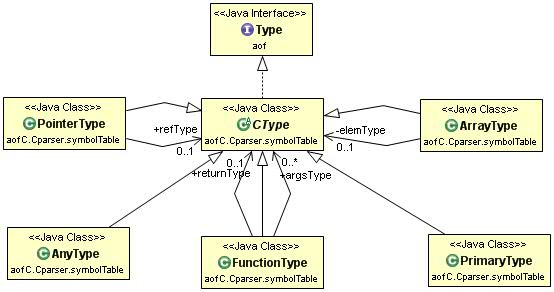
\includegraphics[scale=0.7]{images/AOFC/CType.jpg}
\caption{UML diagram of the CType class and its subclesses.}
\label{fig:CType}
\end{figure}
\\
A complete overview of the language in EBNF notation can be seen in listing \ref{lst:SmallC_EBNF}. Examples of the language will be given later, when each part is explained.\\
\begin{lstlisting}[caption=EBNF notation of the aspect langauge, label=lst:SmallC_EBNF]
file ::= (WS | order | pointcut | advice)* EOF
pointcut ::= 'pointcut' WS NAME WS? '(' args ')' WS? '{' rules '}'
rules ::= (WS | method | member)*
member ::= ('set' | 'get') WS type WS NAME WS? ';'
method ::= ('call' | 'execute') WS type WS NAME WS? '(' args ')' WS? ';'
advice ::= ('advice' WS NAME WS? ':' WS? )? ('before' | 'after' | 'around') WS NAME WS? '(' args ')' WS? '{' .* '}' 
order ::= 'order' WS? '{' WS? NAME (WS? ';' WS? NAME)* WS? '}' 
args ::= (type (WS NAME)? (WS? ',' WS? type (WS NAME)? )* )?
type ::= NAME ('[' ']' | '*')?

NAME ::= (LETTER | SPECIALCHARS | '..') (LETTER | DIGIT | SPECIALCHARS | '..')* 
WS ::= (' ' | '\n' | '\t' | '\r')+
OTHERCHARS ::= ~(LETTER | DIGIT | SPECIALCHARS)
DIGIT ::= '0..9'
LETTER ::= ('a..z' | 'A..Z')
SPECIALCHARS ::= ('*' | '_')
\end{lstlisting}

\section{Pointcuts}
The join points are mapped to pointcuts in a one-on-one manner. For each join point there exists a pointcut, being MethodPointcut and MemberPointcut. The different types are handled by adding a flag to the pointcut to indicate the type. Because identifying a method or a global variable is totally different we need to separate these two. But because a call and an execution both execute on a method we can combine these two together. This also holds for the get and set of a global variable.\\
\\
To identify a method join point we need the signature of the method, consisting of the name of the method, the return type and a set of arguments. Note that the arguments are already implemented by the abstract super class, and thus are not part of the MethodPointcut class. An UML diagram for the MethodPointcut class is shown in figure \ref{fig:MethodPointcut}. Note that wildcards can be used in every element of the pointcut: in the name of the method, as a type of an argument, as  return type or as part of the argument list. It is not allowed to use a wildcard in the name of the arguments since these will be passed on to the advice to be used there, doing this wouldn't make any difference because the arguments are only matched on type and not on name. The names however are used to map them onto the arguments specified in the pointcutset. It is therefor also required that a pointcut contains all the arguments the enclosing pointcutset defines. An example of two method pointcuts are shown in listings \ref{lst:SmallC_MethodPointcutCall} and \ref{lst:SmallC_MethodPointcutExecute}, these pointcuts match respectively the calling and the execution of a method 'mySquare'.\\
\begin{figure}
\centering
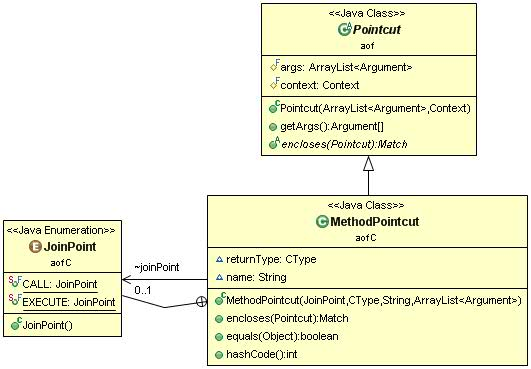
\includegraphics[scale=0.7]{images/AOFC/MethodPointcut.jpg}
\caption{UML diagram of the MethodPointcut class.}
\label{fig:MethodPointcut}
\end{figure}\\
\begin{minipage}{0.42\textwidth}
\begin{lstlisting}[language=C, caption=Example of a method call pointcut, label=lst:SmallC_MethodPointcutCall]
pointcut p() {
	call int mySquare(int);
}
\end{lstlisting}
\end{minipage}\hfill
\begin{minipage}{0.42\textwidth}
\begin{lstlisting}[language=C, caption=Example of a method execution pointcut, label=lst:SmallC_MethodPointcutExecute]
pointcut p() {
	execute int mySquare(int);
}
\end{lstlisting}
\end{minipage}
\\
The MemberPointcut is pretty empty, simply because the best way to identify a global variable is to see it as an argument of the pointcut. By doing this the only thing the MemberPointcut class has to add is the flag to identify the different types, as can be seen in the UML shown in figure \ref{fig:MemberPointcut}. Just as with the MethodPointcut it is possible to use a wildcard as type, but it is also allowed to specify a wildcard as (part of) the name of the member to match multiple global variables. Because a MemberPointcut only contains one argument, being the member, it is always this argument that is mapped to the pointcutset arguments. An example of two member pointcuts are shown in listings \ref{lst:SmallC_MemberPointcutGet} and \ref{lst:SmallC_MemberPointcutSet}, these pointcuts match respectively the getting and setting of a global variable 'count'.\\
\begin{figure}
\centering
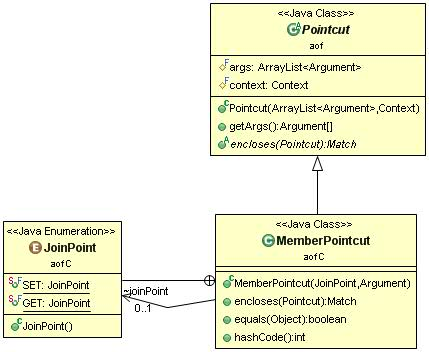
\includegraphics[scale=0.7]{images/AOFC/MemberPointcut.jpg}
\caption{UML diagram of the MemberPointcut class.}
\label{fig:MemberPointcut}
\end{figure}\\
\begin{minipage}{0.42\textwidth}
\begin{lstlisting}[language=C, caption=Example of a member get pointcut, label=lst:SmallC_MemberPointcutGet]
pointcut p() {
	get int count;
}
\end{lstlisting}
\end{minipage}\hfill
\begin{minipage}{0.42\textwidth}
\begin{lstlisting}[language=C, caption=Example of a member set pointcut, label=lst:SmallC_MemberPointcutSet]
pointcut p() {
	set int count;
}
\end{lstlisting}
\end{minipage}
\\
The current implementation does not use the context of the framework, which limits usability. Yet I am convinced that adding a context would not add much functionality since the only context in Small C is the call hierarchy. Note that due to the lack of a context in the pointcuts the method call and execution pointcut will yield the same result, with a context we could for instance get the current method.

\section{Advice}
The advice of our aspect oriented version of Small C is very basic, it contains a string which represents Small C code. The code is allowed to contain arguments that are defined by the pointcutset it is linked to, but these are not treated specially in the CAdvice class itself. Besides the code, the CAdvice class also contains some timing information, as can be seen in figure \ref{fig:CAdvice}. This breaks the clear separation between pointcuts and advice and can be considered to be bad programming, yet this way we can create pointcutsets that are more re-usable. The different types, specifying the moment of execution, are before, after and around. These are the same as are present in AspectJ, and are pretty straightforward. Though while the before and after can only be used to add extra code, the around advice can be used to skip the original code, or modify the values of the parameters. The \textbf{proceed()} call can be used to jump to the original join point (or the next advice, if any). Join points getting or setting a global variable are seen as a typical getter or setter. Note that if the join point has a return type, either a method with a return type or a getter for a variable, the value will be returned by the \textbf{proceed()} call and it is the responsibility of the user to capture this.
\begin{figure}
\centering
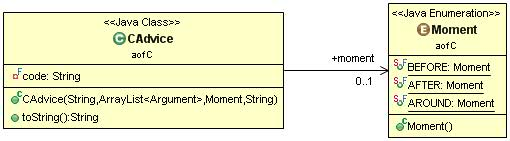
\includegraphics[scale=0.7]{images/AOFC/CAdvice.jpg}
\caption{UML diagram of the CAdvice class.}
\label{fig:CAdvice}
\end{figure}\\
\begin{minipage}{0.42\textwidth}
\begin{lstlisting}[language=C, caption=Example of a before advice, label=lst:SmallC_BeforeAdvice]
advice b: before p() {
	printf("Advice B\n");
}
\end{lstlisting}
\begin{lstlisting}[language=C, caption=Example of an after advice, label=lst:SmallC_AfterAdvice]
advice a: after p() {
	printf("Advice A\n");
}
\end{lstlisting}
\end{minipage}\hfill
\begin{minipage}{0.42\textwidth}
\begin{lstlisting}[language=C, caption=Example of an around advice, label=lst:SmallC_AroundAdvice]
advice c: around p() {
	printf("BEGIN C!\n");
	proceed();
	printf("END C!\n");
}
\end{lstlisting}
\end{minipage}\\
An advice needs to be linked with a pointcutset, this is done by referring to it's name and specifying the arguments it requires. Note that the arguments need to match on type, but may differ on name, the names used in the advice can be used in the body of the advice.\\
\\
The body of the advice is not parsed in any way, at the moment it is created. It is not even parsed anywhere in the entire process until the very end which is simply compiling the weaved code.

\section{Order}
There are two situations in which multiple advices can be mapped to the same moment in execution. The most obvious situation is when multiple advices are linked to the same pointcut set, but also if we have multiple pointcutsets that happen to match the same join point. In both cases it is possible that advices give rise to conflicts, but only if their types overlap.\\
\\
First of all we will discuss the natural order of the advices. If there is no conflict the order is determined by the type of the advice, if there is a conflict but no order, it's up to the framework to resolve it. The location of the advices compared to the join point are shown in figure \ref{fig:COrder}. An overview of all the possible conflicts is more convienently shown in table \ref{tab:SmallC_Conflicts}.
\begin{figure}
\centering
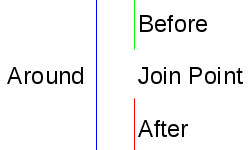
\includegraphics[scale=0.7]{images/AOFC/Order.png}
\caption{The location of the advices.}
\label{fig:COrder}
\end{figure}\\
\begin{table}
\centering
\begin{tabular}{l|c|c|c|}
& before & after & around\\
\hline
before & + & - & + \\
\hline
after & - & + & + \\
\hline
around & + & + & +\\
\hline
\end{tabular}
\caption{An overview of the possible conflicts.}
\label{tab:SmallC_Conflicts}
\end{table}\\
To determine the order when conflicts do arise it is possible to specify an order between any two advices, even those that can never cause a conflict. This may seem useless, but it becomes useful in the case where you want more than two advice to be in a specific order and they are of different types. An order is specified as a list of advices, in which a later advice is closer to the join point then an earlier one. An example of specifying an order is shown in listing \ref{lst:SmallC_OrderExample} and listing \ref{lst:SmallC_OrderExampleResult}, in this example \textit{jp} is used to denote the join point. The order specified here compares a before and after advice but will have no effect as they can never cause a conflict. Note that it is possible to switch the before and after advice in the order and still get the same result.\\
\begin{minipage}{0.42\textwidth}
\begin{lstlisting}[language=C, caption=An example of a non-trivial order, label=lst:SmallC_OrderExample]
order{c; b; a}

advice b: before p() {
	printf("Advice B\n");
}

advice a: after p() {
	printf("Advice A\n");
}

advice c: around p() {
	printf("BEGIN C!\n");
	proceed();
	printf("END C!\n");
}
\end{lstlisting}
\end{minipage}\hfill
\begin{minipage}{0.42\textwidth}
\begin{lstlisting}[language=C, caption=The result of the order, label=lst:SmallC_OrderExampleResult]
printf("BEGIN C!\n");
printf("Advice B\n");
jp;
printf("Advice A\n");
printf("END C!\n");
\end{lstlisting}
\end{minipage}\\

\section{Weaver}
The weaver is the biggest piece of code, after all it is the core part of every aspect oriented language. Once it has all the information it can start putting it together, it does this by writing wrapper methods for the join points, even if there is no advice to be execute for this join point. This last could have been omitted, but for simplicity it is not. Which wrappers are generated depends on the join point, and partly on the advices. For every global variable declared there will be two wrappers, one to handle the access to the variable, and another for the assignment of a new value. The same holds for a method but with call and execution instead. Two examples of these wrappers are shown in listing \ref{lst:SmallC_WrapperVariable} and \ref{lst:SmallC_WrapperMethod}. The original operations will be modified so that they use the wrappers instead. Two examples of these changes are shown in listing \ref{lst:SmallC_WrapperUsageBefore} and \ref{lst:SmallC_WrapperUsageAfter}.\\
\begin{minipage}{0.45\textwidth}
\begin{lstlisting}[language=C, caption=Example of variable wrappers, label=lst:SmallC_WrapperVariable]
int count_get_() {
	int _result_;
	_result_ = count;
	return _result_;
}

void count_set_(int _new_) {
	count = _new_;
}
\end{lstlisting}
\end{minipage}\hfill
\begin{minipage}{0.45\textwidth}
\begin{lstlisting}[language=C, caption=Example of method wrappers, label=lst:SmallC_WrapperMethod]
int mySqrt_exec_(int a) {
	int _result_;
	_result_ = mySqrt(a);
	return _result_;
}

int mySqrt_call_(int a) {
	int _result_;
	_result_ = mySqrt_exec_(a);
	return _result_;
}
\end{lstlisting}
\end{minipage}\\
\begin{minipage}{0.45\textwidth}
\begin{lstlisting}[language=C, caption=Example of code before weaving, label=lst:SmallC_WrapperUsageBefore]
x = mySqrt(25);
count = count + 1;
x = mySquare(count);
\end{lstlisting}
\end{minipage}\hfill
\begin{minipage}{0.45\textwidth}
\begin{lstlisting}[language=C, caption=Example of code after weaving, label=lst:SmallC_WrapperUsageAfter]
x = mySqrt_call_(25);
count_set_(count_get_() + 1);
x = mySquare_call_(count_get_());
\end{lstlisting}
\end{minipage}\\
Besides these wrappers some other methods are generated as well. One for each advice of the type before or after, and one for each matching join point of an around advice. The reason the around advices needs multiple instances is that it will have to proceed to the original method. While this is not the case for the before and after advice, it is still much easier to put them in a separate method, especially if you consider that such an advice can alter the values of arguments, but that these changes may not be passed on to the actual method, only the around advice may do such things. The generated methods are those that are generated for the advice specified in listings \ref{lst:SmallC_BeforeAdvice}, \ref{lst:SmallC_AfterAdvice} and \ref{lst:SmallC_AroundAdvice}.\\
\begin{lstlisting}[language=C, caption=Generated methods, label=lst:SmallC_GeneratedMethods]
void _a() {
	printf("Advice A\n");
}

void _b() {
	printf("Advice B\n");
}

void _c_myMethod_() {
	printf("BEGIN C!\n");
	{
		 myMethod();
	}
	printf("END C!\n");
}
\end{lstlisting}
Besides generating wrappers, the weaver is also responsible for delivering the right arguments to the advice, this is another situation that shows the advantages of putting an advice in a separate method. The around advice also contains a proceed() call, the weaver has to replace this with a call to the original method or next around advice. The arguments specified in the proceed must be conserved and passed on. To not complicate the weaver any further it is required that the user manages the declaration of a value to store the return result and explicitly returns this value if a return value is required. The declaration, assigning the return value of the proceed() and return the value all must occur separately. This is because it is possible that the weaver will insert calls to other advices before and after the proceed call. An example of this is shown in listing \ref{lst:SmallC_ComplexAround}, where the around advice is generated using the order as specified in listing \ref{lst:SmallC_OrderExample}.\\
\begin{lstlisting}[language=C, caption=A generated method for an around advice with advice nested within, label=lst:SmallC_ComplexAround]
int _c_mySquare_(int a) {
	int retVal = 0;
	printf("BEGIN C!\n");
	{
		_b();
		retVal = mySquare(a);
		_a();
	}
	printf("END C!\n");
	return retVal;
}
\end{lstlisting}
\begin{figure}
\centering
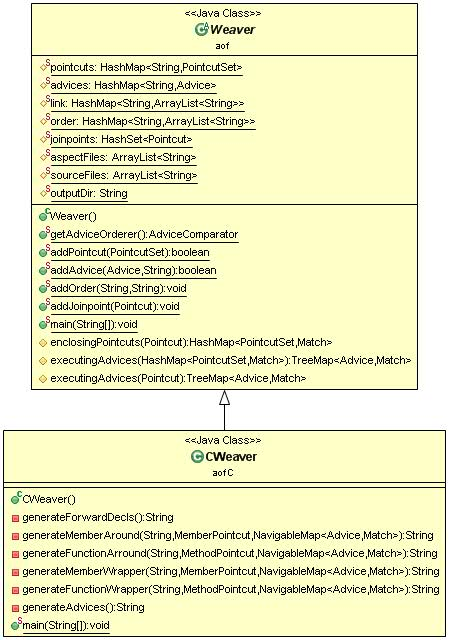
\includegraphics[scale=0.7]{images/AOFC/CWeaver.jpg}
\caption{UML diagram of the CWeaver class.}
\label{fig:CWeaver}
\end{figure}
Now that all the components have been introduced, I give a final overview of the entire structure in figure \ref{fig:CFull} to make it extra clear how all the components are connected.
\begin{figure}
\centering
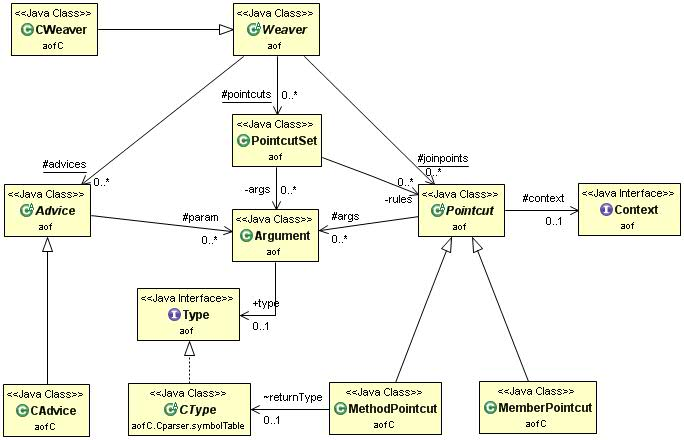
\includegraphics[scale=0.55]{images/AOFC/CFull.jpg}
\caption{A full overview of the use of the framework for Small C.}
\label{fig:CFull}
\end{figure}

\section{Example}
In this section a complete example is shown to get a better feeling of how all the pieces fit together.
\begin{lstlisting}[language=C, multicols=2, caption=Source code, label=lst:SmallC_ExampleSource]
#include <stdio.h>

int count = 0;

/* a^b */
int myPow(int a, int b) {
	int x;
	int result = 1;
	
	if (b <= 0) {
		return 1;
	}
	
	for (x = 1; x <= b; x = x + 1) {
		result = result * a;
	}
	
	return result;
}

/* a^2 */
int mySquare(int a) {
	return a * a;
}

/* square root of a. */
int mySqrt(int a) {
	int i = 1;
	while (mySquare(i) <= a) {
		i = i + 1;
	}
	
	return i - 1;
}

/* b-th root of a. */
int myRoot(int a, int b) {
	int i = 1;
	while (myPow(i, b) <= a) {
		i = i + 1;
	}
	
	return i - 1;
}

/* log_b(a) */
int myLog(int a, int b) {
	int i = 1;
	while (myPow(b, i) <= a) {
		i = i + 1;
	}
	
	return i - 1;
}

void main () {
	int a = 2;
	int b = 10;
	
	int x = myPow(a, b);
	count = count + 1;
	x = mySquare(a);
	count = count + 1;
	x = mySqrt(a);
	count = count + 1;
	x = mySqrt(25);
	count = count + 1;
	x = myRoot(1024, 2);
	count = count + 1;
	x = myLog(1024, 2);
	count = count + 1;
	x = mySquare(count);
}
\end{lstlisting}
\begin{lstlisting}[language=C, multicols=2, caption=The aspect code.]
order{b; c; a}

pointcut p(int x) {
	call int my..(int x, ..);
}

pointcut q(int i) {
	call int random(int i);
}

pointcut v(int count) {
	get int count;
}

advice getv: before v(int i) {
	printf("Count = %i\n", i);
}

advice a: after p(int i) {
	printf("BEGIN A\n");
}

advice b: after p(int i) {
	printf("BEGIN B\n");
}

advice c: around p(int i) {
	int retVal = 0;
	printf("BEGIN C!\n");
	retVal = proceed(i);
	printf("END C!\n");
	return retVal;
}
\end{lstlisting}
\begin{lstlisting}[language=C, multicols=2, caption=Weaved code]
#include <stdio.h>

int count = 0;
int myPow(int a, int b) {
	int x = 0;
	int result = 1;
	if (b <= 0) {
		return 1;
	}
	
	for (x = 1; x <= b; x = x + 1) {
		result = result * a;
	}
	
	return result;
}

int mySquare(int a) {
	return a * a;
}

int mySqrt(int a) {
	int i = 1;
	while(mySquare_call_(i) <= a) {
		i = i + 1;
	}
	
	return i - 1;
}

int myRoot(int a, int b) {
	int i = 1;
	while(myPow_call_(i, b) <= a) {
		i = i + 1;
	}
	
	return i - 1;
}

int myLog(int a, int b) {
	int i = 1;
	while(myPow_call_(b, i) <= a) {
		i = i + 1;
	}
	
	return i - 1;
}

void main() {
	int a = 2;
	int b = 10;
	int x = myPow_call_(a, b);
	count_set_(count_get_() + 1);
	x = mySquare_call_(a);
	count_set_(count_get_() + 1);
	x = mySqrt_call_(a);
	count_set_(count_get_() + 1);
	x = mySqrt_call_(25);
	count_set_(count_get_() + 1);
	x = myRoot_call_(1024, 2);
	count_set_(count_get_() + 1);
	x = myLog_call_(1024, 2);
	count_set_(count_get_() + 1);
	x = mySquare_call_(count_get_());
}

void _getv(int i) {
	printf("Count = %i\n", i);
}

void _b(int i) {
	printf("BEGIN B\n");
}

void _a(int i) {
	printf("BEGIN A\n");
}

int count_get_() {
	int _result_;
	_getv(count);
	_result_ = count;
	return _result_;
}

int myPow_exec_(int a, int b) {
	int _result_;
	_result_ = myPow(a, b);
	return _result_;
}

void main_call_() {
	main_exec_();
}

int myLog_exec_(int a, int b) {
	int _result_;
	_result_ = myLog(a, b);
	return _result_;
}

int _c_myLog_(int i, int b) {
	int retVal = 0;
	printf("BEGIN C!\n");
	{
		retVal = myLog_exec_(i, b);
		_a(i);
	}

	printf("END C!\n");
	return retVal;
}

int myLog_call_(int a, int b) {
	int _result_;
	_result_ = _c_myLog_(a, b);
	_b(a);
	return _result_;
}

int mySqrt_exec_(int a) {
	int _result_;
	_result_ = mySqrt(a);
	return _result_;
}

int _c_myRoot_(int i, int b) {
	int retVal = 0;
	printf("BEGIN C!\n");
	{
		retVal = myRoot_exec_(i, b);
		_a(i);
	}

	printf("END C!\n");
	return retVal;
}

int myRoot_call_(int a, int b) {
	int _result_;
	_result_ = _c_myRoot_(a, b);
	_b(a);
	return _result_;
}

int mySquare_exec_(int a) {
	int _result_;
	_result_ = mySquare(a);
	return _result_;
}

int _c_mySqrt_(int i) {
	int retVal = 0;
	printf("BEGIN C!\n");
	{
		retVal = mySqrt_exec_(i);
		_a(i);
	}

	printf("END C!\n");
	return retVal;
}

int mySqrt_call_(int a) {
	int _result_;
	_result_ = _c_mySqrt_(a);
	_b(a);
	return _result_;
}

int _c_myPow_(int i, int b) {
	int retVal = 0;
	printf("BEGIN C!\n");
	{
		retVal = myPow_exec_(i, b);
		_a(i);
	}

	printf("END C!\n");
	return retVal;
}

int myPow_call_(int a, int b) {
	int _result_;
	_result_ = _c_myPow_(a, b);
	_b(a);
	return _result_;
}

void main_exec_() {
	main();
}

int myRoot_exec_(int a, int b) {
	int _result_;
	_result_ = myRoot(a, b);
	return _result_;
}

void count_set_(int _new_) {
	count = _new_;
}

int _c_mySquare_(int i) {
	int retVal = 0;
	printf("BEGIN C!\n");
	{
		retVal = mySquare_exec_(i);
		_a(i);
	}

	printf("END C!\n");
	return retVal;
}

int mySquare_call_(int a) {
	int _result_;
	_result_ = _c_mySquare_(a);
	_b(a);
	return _result_;
}
\end{lstlisting}

\section{Difficulties}
Despite having a modifiable compiler, there were a lot of problems of weaving the advices into the code. This was caused by the fact that the compiler was not designed to allow changes after parsing the code. Changing this would require big changes in the compiler and was therefor not really an option. Instead of changing the compiler another alternative was used, by creating two compilers, both with small changes, we could weave the file in multiple passes.\\
\\
In phase 1 the source code will be parsed and all join points will be specified to the weaver. The weaver will produce wrappers and add these to a temporary output file. In phase 2 the modified file will be parsed and the original calls will be modified to point to the wrappers. In phase 3 the actual advice bodies will be written to the wrappers. Phase 4 is to compile the weaved file with a regular compiler, this is not done by the weaver and has to be done by the user himself.\\
\\
It was impossible to change the calls in the first phase due to a simple circular dependency. The compiler checks that the called function actually exists. Since the compiler does not allow to add declarations before the current point, these declarations have to exist in the source code itself. To do this however we need to know which join points occur, and thus we need to have parsed the file before.\\
\\
Adding the content can not be done before phase 2, simply because the content contains function calls to the actual functions which need to be kept. It is impossible to distinguish a call from within a wrapper from one within a 'normal' function, yet we need to treat them separately. Therefor we need to add the content in a separate phase.

\chapter{Dot}
\label{chap:Dot}
Dot is a language that allows you to easily specifies the structure and appearance of a graph. Some of the features the language supports  are directed edges, undirected edges, subgraphs, labels for nodes and edges, different shapes, colors and more. Despite that it is a pretty simple to use language, and has a very straightforward syntax it tends to be very verbose when trying to create large and complicated graphs.\\
\\
Dot does not have any time related aspect as the result of the 'compiler' is the graph that the user wants. Because of this it adding AOP may seem weird since join points are defined as points in the execution of a program. Since the program does not execute, but is a static graph, all the join points simply map to points in the code in a static way. Yet the ideas of AOP can still be applied.\\
\\
Because the syntax of Dot is that self-explaining, the example showed in listing \ref{lst:Dot_Example} and the resulting graph in figure \ref{fig:Dot_Example} is enough to get an understanding of the language.\\
\begin{figure}
\begin{minipage}{0.45\textwidth}
\begin{lstlisting}[caption=The code to create a graph, label=lst:Dot_Example]
digraph G {
	subgraph cluster_0 {
		style=filled;
		color=lightgrey;
		node [style=filled,color=white];
		a0 -> a1 -> a2 -> a3;
		label = "process #1";
	}

	subgraph cluster_1 {
		node [style=filled];
		b0 -> b1 -> b2 -> b3;
		label = "process #2";
		color=blue
	}
	
	start -> a0;
	start -> b0;
	a1 -> b3;
	b2 -> a3;
	a3 -> a0;
	a3 -> end;
	b3 -> end;

	start [shape=Mdiamond];
	end [shape=Msquare];
}
\end{lstlisting}
\end{minipage}\hfill
\begin{minipage}{0.45\textwidth}
\centering
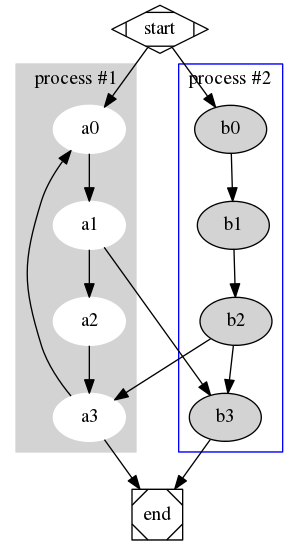
\includegraphics[width=\linewidth]{images/AOFDot/SmallExample.png}
\caption{The generated graph by dot.}
\label{fig:Dot_Example}
\end{minipage}
\end{figure}

\section{Join Point Model}
The join points identified in Dot are all the elements of the graph, being the graph itself, nodes and edges. This simple join point model is mostly caused by the lack of run-time behavior.

\section{Base Language Compiler}
The compiler for the base language contained a parser that made it possible to request all the graphs, nodes, and edges present in the file. Because of this no modifications were made to the base parser.

\section{Aspect Language}
The aspect language mostly uses the same syntax as Dot itself to keep the language as simple as possible. There exists a wildcard to create more general rules, being '..'. By using this the programmer specifies that anything can take its place.\\
\\
Just as in Dot itself an graph, node and edge can contain attributes, these attributes are considered to be the arguments of the element and are used to restrict the matching. An attribute needs to have a name, being the attribute itself, though the value can be the wildcard. It is also important to note that the wildcard can be used to denote any other attribute, without this only elements with exactly those attributes are matched. Note that these attributes only act as arguments for the element and not for the pointcut.\\
\\
It are the elements that can be used as arguments, but to prevent having to make an entire type system for it, the id's of the elements are used instead. This makes it possible to keep the type system very basic, as can be seen in figure \ref{fig:DotType}.
\begin{figure}[h]
\centering
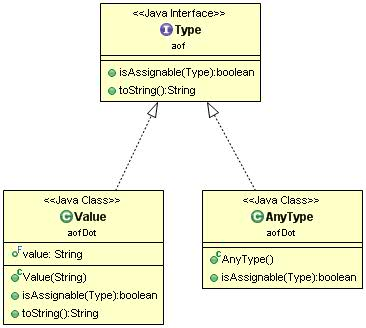
\includegraphics[scale=0.7]{images/AOFDot/DotType.jpg}
\caption{UML diagram of the type system for aspect orientation in Dot.}
\label{fig:DotType}
\end{figure}\\
There is no context information used, though it is possible to match elements based on the greater picture, being the graph they are part of. This will become clear when explaining the pointcuts and more specific the GraphPointcut.\\
\\
A complete overview of the language in EBNF notation is shown in listing \ref{lst:Dot_EBNF}.
\begin{lstlisting}[caption=EBNF notation of the aspect language., label=lst:Dot_EBNF]
file ::= (WS | order | pointcut | advice)* EOF
order ::= 'order' WS? '{' WS? NAME (WS? ';' WS? NAME)* WS? '}'
pointcut ::= 'pointcut' WS NAME WS? '(' args ')' WS? '{' rules '}' 
advice ::= ('advice' WS NAME WS? ':' WS? )? ('insert' | 'delete') WS NAME WS? '(' args ')' WS? '{' rules '}'
args ::= (WS? type WS NAME (WS? ',' WS? type WS NAME)* WS? )?

rules ::= (WS | graph | node ';' | edge ';')*
graph ::= ('..graph' | 'graph' | 'digraph' | 'subgraph') WS (NAME | '..') WS? '{' rules '}'
edge ::= (NAME WS? '=' WS? )? '(' WS? node WS? ')' WS? ('->' | '--') WS? '(' WS? node WS? ')' (WS? '[' attributes ']')?
node ::= (NAME | '..') (WS? '=' WS? (NAME | '..'))? (WS? '[' attributes ']')?
attributes ::= (NAME WS? '=' WS? (NAME | '..') (WS? ',' WS? attributes)? | '..')
type ::= ('Node' | 'Edge' | 'Graph')

NAME ::= '..'? ((LETTER | DIGIT | '_' | '"' .* '"') '..'? )* 
WS ::= (' ' | '\n' | '\t' | '\r')+
DIGIT ::= '0..9'
LETTER ::= ('a..z' | 'A..Z')
\end{lstlisting}

\section{Pointcuts}
Every join point is expressed by a pointcut, resulting in three pointcuts being GraphPointcut, NodePointcut and EdgePointcut which represent respectively a graph, node and edge. All of these pointcuts can have Dot attributes, these will be stored as arguments and thus are part of the superclass Pointcut. But because each pointcut also has specific information I will now discuss these three pointcuts into more detail.\\
\\
The GraphPointcut requires all the information of it's nodes and edges. Instead of introducing new types for nodes and edges, it is easier to reuse the pointcuts to represent this. A graph also has a name, though this information is not used in the current version.\\
Checking whether a graph matches with a GraphPointcut is very simple, we just need to compare the nodes and edges it contains, which is discussed when we introduce these pointcuts and we need to verify that all the attributes are present and have the same value if any specified. A wildcard can be used to indicated that the graph may contain more nodes and edges, or that the attributes is just a subset. An example of a graph pointcut is shown in listing \ref{lst:Dot_GraphPointcut}.
\begin{lstlisting}[caption=A graph pointcut matching any graph G with an edge from start to main, label=lst:Dot_GraphPointcut]
pointcut n() {
	graph G {
		(start [..] ->  main [..]) [..];
		.. [..];
		(.. [..]) -> (.. [..]) [..];
	}
}
\end{lstlisting}
A NodePointcut is the easiest as it only has a name and attributes, and since attributes are already handled by the superclass all we need to do is add a name. A node matches a NodePointcut if it has the same name and all the attributes match. An example of such a node poincut is shown in listing \ref{fig:Dot_NodePointcut}.
\begin{lstlisting}[caption=A node pointcut matching any node start, label=lst:Dot_NodePointcut]
pointcut n() {
	start [..];
}
\end{lstlisting}
An EdgePointcut isn't that much harder, thanks to the compiler every edge contains exactly two nodes: a source and a target. These two nodes are again represented by a NodePointcut, as this was the easiest solution. On top of that we also need to know whether the edge is directed or not, which is a simple boolean. An edge matches a pointcut if they are either both directed and the sources and targets match, if they are both undirected the source and target node may be switched. An example of an edge pointcut is shown in listing \ref{fig:Dot_EdgePointcut}.
\begin{lstlisting}[caption=An edge pointcut matching any edge from start to main, label=lst:Dot_EdgePointcut]
pointcut n() {
	(start [..]) -> (main [..]) [..];
}
\end{lstlisting}
An overview of all the pointcuts and their interaction is shown in figure \ref{fig:DotPointcuts}.
\begin{figure}
\centering
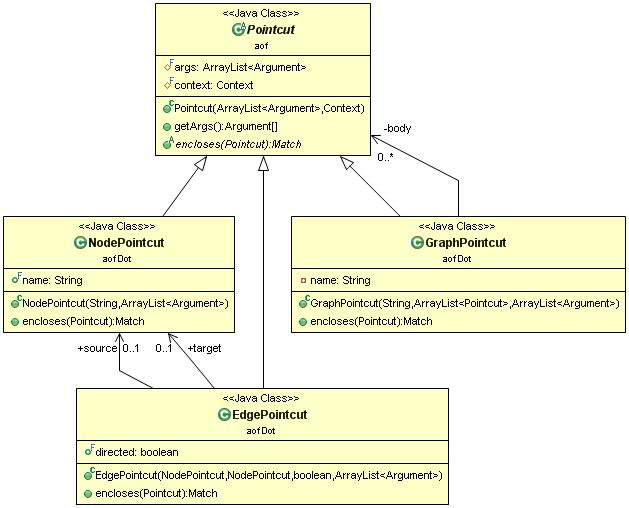
\includegraphics[scale=0.6]{images/AOFDot/DotPointcuts.jpg}
\caption{UML diagram of the three pointcut classes.}
\label{fig:DotPointcuts}
\end{figure}
\\
The current version does not use the context mechanism, but the user can specify that a form of context by wrapping it in a graph. By doing this, we can make a link between different elements in the same graph. I believe that this is also the only possible use for a context in Dot.\\
\\
Parameters can be introduced on every level of the pointcut, this is shown by the examples in listing \ref{lst:Dot_Arguments}. Though the pointcut expresses the type of the argument, this is not really used by the weaver. As mentioned earlier it is the id of the elements that are used internally.
\begin{lstlisting}[caption=Examples showing the use of arguments, label=lst:Dot_Arguments]
pointcut n(Edge i, Node j) {
	graph .. {
		i = (main [..]) -> (j = .. [..]) [..];
		.. [..];
		(.. [..]) -> (.. [..]) [..];
	}
}

pointcut o(Node i) {
	i = .. [..];
}

pointcut p(Edge i) {
	i = (main [..]) -> (.. [..]) [..];
}
\end{lstlisting}

\section{Advice}
There exists two kinds of advice: insert and delete, which are meant to respectively insert elements or delete them from the pointcut. It is possible to add attributes to an element simply by creating an element that already exists. Modifying an attribute is done in the same way. Deleting an attribute is done by specifying an attribute next to the element, if no such attribute is specified the entire element id deleted. Using arguments is possible to specify the elements that were matched in the pointcut. To provide this functionality the DotAdvice is created, this contains the type of the advice and the body, being the elements that have to be inserted or deleted. These elements are expressed using the Pointcuts, this allows us to quickly re-use all the functionality for the pointcuts, among which the usage of parameters and wildcards. An example of an advice is shown in figure \ref{lst:Dot_Advice}.\\
\begin{figure}
\centering
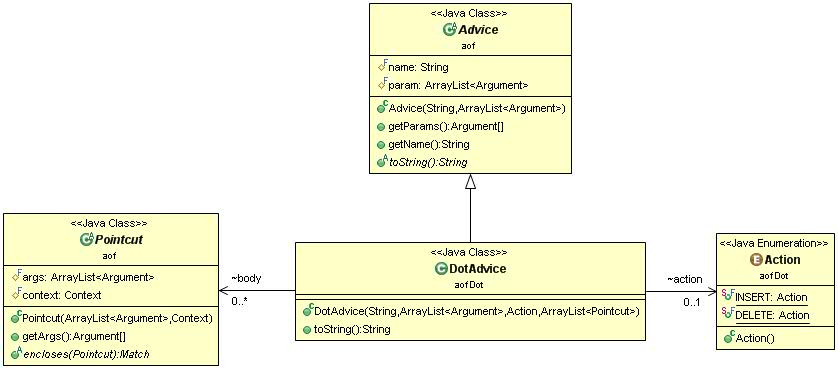
\includegraphics[scale=0.6]{images/AOFDot/DotAdvice.jpg}
\caption{UML diagram of the DotAdvice class.}
\label{fig:DotAdvice}
\end{figure}
\\
\begin{lstlisting}[caption=An example of advice., label=lst:Dot_Advice]
advice fn: insert n() {
	main [shape=box];
}

advice dn: delete n() {
	main [color=..];
}

advice in: insert n(Node i) {
	i [shape=box];
}

advice ie: insert n() {
	(main) -> (exit);
}
\end{lstlisting}

\section{Order}
Despite the absence of runtime behaviour it is still possible that conflicts arise if two advices modify the same element and the modifications overlap. Just think of an advice that colors a node red, and another that colors it blue. By changing the order of these two advices we either get a red node or a blue one. To specify an order, we simply create a point-comma separated list of the order in which they have to be executed. If there are two advices without an order that do execute at the same time, the order is undetermined. An example of the order is shown in listing \ref{lst:Dot_Order}.
\begin{lstlisting}[caption=An example of the order., label=lst:Dot_Order]
order{dn; fn}

pointcut n(Node i) {
	i = .. [..];
}

advice dn: delete n(Node i) {
	i [color=..];
}

advice fn: insert n(Node i) {
	i [color="0.000 1.000 1.000"];
}
\end{lstlisting}

\section{Weaver}
The weaver will first gather all advices and after that it will start executing them. This is important as it means that if one advice modifies an element in such a way that it no longer matches a pointcut any changes caused by advices liked to that pointcut will still be executed.\\
\\
No other important notes are to be made. Thanks to the Dot compiler it is easy to get all the graphs, nodes and edges from a file modify them and write the resulting graph back to file.\\
\begin{figure}
\centering
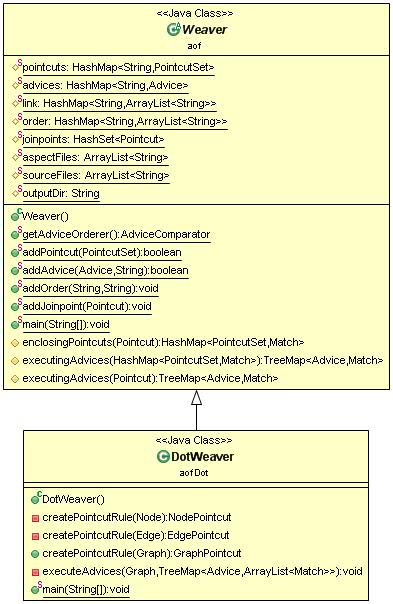
\includegraphics[scale=0.7]{images/AOFDot/DotWeaver.jpg}
\caption{UML diagram of the DotWeaver class.}
\label{fig:DotWeaver}
\end{figure}

\section{Example}
Now that all the basic elements are explained it is time to show a more complicated example. I will provide both the code and the visual graph before and after the weaving.
\begin{lstlisting}[multicols=2, caption=The source code.]
digraph finite_state_machine {
	rankdir=LR;
	node [shape = circle];

	LR_0 [shape = doublecircle];
	LR_3 [shape = doublecircle];
	LR_4 [shape = doublecircle]
	LR_8 [shape = doublecircle];

	LR_0 -> LR_2 [label = "SS(B)"];
	LR_0 -> LR_1 [label = "SS(S)"];
	LR_1 -> LR_3 [label = "S($end)"];
	LR_2 -> LR_6 [label = "SS(b)"];
	LR_2 -> LR_5 [label = "SS(a)"];
	LR_2 -> LR_4 [label = "S(A)"];
	LR_5 -> LR_7 [label = "S(b)"];
	LR_5 -> LR_5 [label = "S(a)"];
	LR_6 -> LR_6 [label = "S(b)"];
	LR_6 -> LR_5 [label = "S(a)"];
	LR_7 -> LR_8 [label = "S(b)"];
	LR_7 -> LR_5 [label = "S(a)"];
	LR_8 -> LR_6 [label = "S(b)"];
	LR_8 -> LR_5 [label = "S(a)"];
}
\end{lstlisting}
\begin{figure}
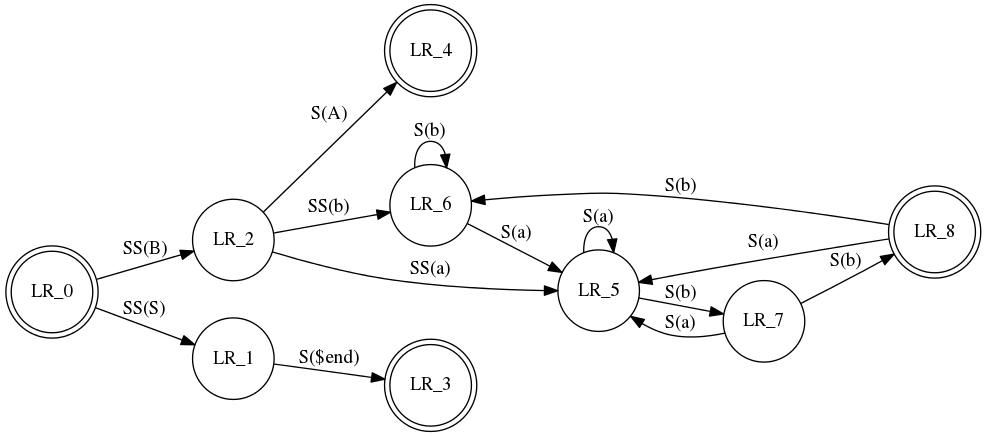
\includegraphics[width=\textwidth]{images/AOFDot/ExampleBefore.png}
\caption{The graph before weaving.}
\end{figure}
\begin{lstlisting}[multicols=2, caption=Aspect code.]
order{fn; color}

pointcut n(Node j) {
	j = LR_.. [..];
}

pointcut m(Edge j) {
	j = (.. [..]) -> (.. [shape=doublecircle, ..]) [..];
}

pointcut end(Node n) {
	n = .. [shape=doublecircle];
}

advice fn: insert n(Node j) {
	j [color=blue];
}

advice mark: insert m(Edge j) {
	j [color=red];
}

advice color: delete end(Node n) {
	n [color=..];
}

advice shape: insert end(Node n) {
	n [shape=box];
}
\end{lstlisting}
\begin{figure}
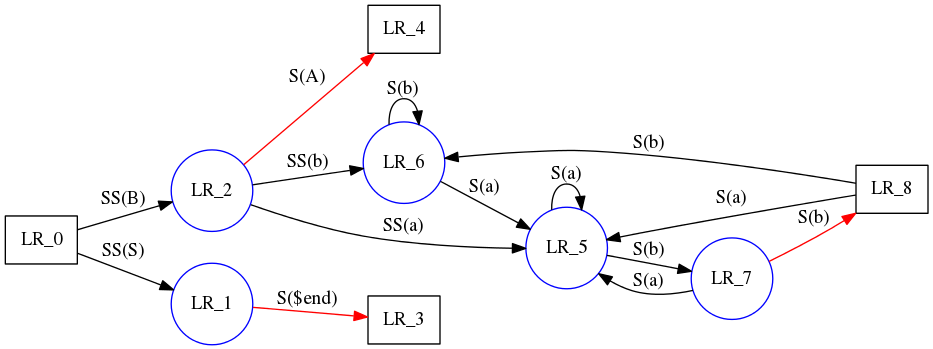
\includegraphics[width=\textwidth]{images/AOFDot/ExampleAfter.png}
\caption{The graph after weaving.}
\end{figure}

\section{Difficulties}
The biggest problem encountered was how to decide on the syntax of the aspect language. Once this was done adding aspect orientated programming went really fast, also thanks to the compiler which allowed it to easily modify the graph and write it back to file.\\
\\
One small problem was that there were two minor bugs in the compiler which needed to be fixed first, but this could be done really fast due to the availability of the source code.

\chapter{AOWP}
AOWP \cite{hokamura_aspect-oriented_2008} is a domain specific language for web applications. Most web applications are developed with the Model-View-Controller framework which clearly separates the application into business logic (model layer) and the visual component (view layer), which communicate through the controller. It is however this framework that makes general AOP languages unfeasible as they break this clear separation.\\
\\
Though there exists an AOP language for PHP called AOPHP, this language has some flaws. First of all there is a lack of pointcuts to really cover all join points of web applications. Secondly there is no way to handle a history of page visits without modifying the web pages. Finally we note that the aspects can not be sufficiently separated from the crosscutting concerns.

\section{Join Point Model}
The join points that can occur in a web application consists of events based on HTTP and language specifications of well-known Web programming languages such as PHP and Java/Servlet. Where the first consists of receiving HTTP requests, reading form data and reading or writing cookie data, the latter consists of reading the session data. An overview of all the events is shown in table \ref{tab:AOWP_Events}.
\begin{table}
\centering
\begin{tabular}{l|l}
\hline
Abbreviation & Event\\
\hline
\hline
REQ & Receive an HTTP Request\\
\hline
F/R & Read the form data\\
\hline
C/R & Read the cookie data\\
\hline
C/W & Write the cookie data\\
\hline
S/R & Read the session data\\
\hline
S/W & Write the session data\\
\hline
\end{tabular}
\caption{AOWP events}
\label{tab:AOWP_Events}
\end{table}

\section{Aspect Language}
AOWP re-uses the syntax of web programming languages such as PHP and Java/Servlet. It does this by mapping the aspect constructs on to object oriented structures. By doing this the effort required by the user is minimizes as he doesn't need to learn a new language.\\
\\
Creating an aspect can be done by creating a class that extends the Aspect class, adding a pointcut and an advice is done by declaring functions with the name of respectively 'pointcut' and the name of the type of advice ('before', 'after', 'around'). An example is shown in listing \ref{lst:AOWP_ExampleNews} and \ref{lst:AOWP_ExampleLoad}.\\
\\
This could also be accomplished if we were to use the framework, since it is required to create an aspect language of our own. This means that the same syntax could be chosen, though it has to be said that the framework has no notion of aspects, but this is not a problem as it is the responsibility of the compiler to extract the required information and provide it to the weaver in a format it understands.

\section{Pointcuts}
There are three categories of pointcuts, a first one selects events, a second selects event flows and a third selects based on usage contexts. Each of these categories has a set of sub-types, or so called designators. An overview of all the designators are given in tables \ref{tab:Designators_AOWP_Events}, \ref{tab:Designators_AOWP_Flows} and \ref{tab:Designators_AOWP_Contexts}.
\begin{table}
\centering
\begin{tabular}{l|p{7cm}}
\hline
Designator & Description\\
\hline
\hline
request & Select REQ with the specified URL\\
\hline
getget & Select specified F/R in a GET request\\
\hline
postget & Select specified F/R in a POST request\\
\hline
cookieget & Select specified C/R\\
\hline
cookieset & Select specified C/W\\
\hline
sessionget & Select specified S/R\\
\hline
sessionset & Select specified S/W\\
\hline
\end{tabular}
\caption{Designators for selecting AOWP events}
\label{tab:Designators_AOWP_Events}
\end{table}
\begin{table}
\centering
\begin{tabular}{l|p{7cm}}
\hline
Designator & Description\\
\hline
\hline
withinrequest & Select all AOWP events in a REQ\\
\hline
pflow & Select all AOWP events in specified page transitions\\
\hline
\end{tabular}
\caption{Designators for selecting AOWP event flows}
\label{tab:Designators_AOWP_Flows}
\end{table}
\begin{table}
\centering
\begin{tabular}{l|p{7cm}}
\hline
Designator & Description\\
\hline
\hline
accessnum & Select all AOWP events when the number of access users is the specified number or greater.\\
\hline
\end{tabular}
\caption{Designators based on usage contexts}
\label{tab:Designators_AOWP_Contexts}
\end{table}
How these designators are used can be seen in table \ref{tab:Designators_AOWP_Pointcut}.
\begin{table}
\centering
\begin{tabular}{l|p{7cm}}
\hline
Example & Description\\
\hline
\hline
request(/news.php) & Selects all events of receiving HTTP requests on news.php.\\
\hline
withinrequest(/login.php) & Selects all events generedted during the execution of HTTP requests for login.php\\
\hline
pflow(/news.php) & Selects all the events involved in handling HTTP requests when the user has seen news.php\\
\hline
accessnum(5) & Selects all events involved in handling HTTP Requests when the number of users if 5 or more.\\
\hline
request(/*Action.php) & Selects the REQ whose name starts with '/' and ends with 'Action.php'.\\
\hline
!pflow(/news.php) & Selects a negative set of events selected by pflow(/news.php)\\
\hline
\end{tabular}
\caption{Examples of designator.}
\label{tab:Designators_AOWP_Pointcut}
\end{table}
From this table we also see that it is possible to use regular expressions as an argument of a designator.\\
\\
I will now discuss how these pointcuts could be implemented with the earlier presented framework. Instead of creating a pointcut subclass for each category it is more interesting to only create one subclasses being AOWPPointcut. I choose to take all the pointcuts together as their is no distinction in how these are represented. The class will rely on the arguments of the Pointcut superclass to implement the argument. The specific designator this instance represents has to be indicated by a special value, either an enum or an integer.\\
\\
By doing this we can easily specify pointcuts, creating join points is however a bit more tricky due to capturing the flow. We could do this naivly and create a pointcut for each element along the flow, but that would cause a long delay. It is much better to capture the entire flow as a context and provide that along with the join point. This means that checking whether a pointcut matches a join point is a bit more work, but it allows us to generate only one instance for the entire join point.\\
\\
AOWP allows combining multiple designators by using the negation (!), intersection (\&) and union ($|$) operator. This is not possible with the framework, since this only supports union. It is however not a big problems as we can create a new type of pointcut, the OperatorPointcut. This pointcut will simply execute a certain operator (!, \& or $|$) on its members, which are again pointcuts. Another approach could have been to use the union of the framework and using the OperatorPointcut only for the negation and intersection, but this would lead to some extra work to be done. We would have to rework some expressions to make the unions the top-level operator or remote them completely. This can be seen in the following examples. In these examples I use simple letters to represent pointcuts.\\
\begin{align*}
!\left(a | b\right) \& c & \Rightarrow \left(!a \& !b\right) \& c\\
\left(a | b \right) \& !c & \Rightarrow \left(a \& !c\right) | \left(b \& !c \right)
\end{align*}
To avoid this extra work it makes more sense to treat the union the same way as the negation and the intersection.

\section{Advice}
The types of advice AOWP supports is the same as AspectJ, being 'before', 'after' and 'around'. The body of an advice is normal code. Because this is the same as Small C, which is explained earlier, I will not discuss this here again.

\section{Weaver}
Due to the dynamic behaviour of web applications it is impossible to rely on compile time weaving, and thus run-time weaving is required. The weaver itself works pretty straightforward by extracting join point shadows and injects code to call the weaver.\\
\\
This would cause some problems when using the framework, as the current version does not support run-time weaving. A work-around is to set up the weaver each time it is required, but this introduces a large overhead for creating and loading the pointcuts each time.

\section{Examples}
\begin{lstlisting}[caption=An advice to alert the user to check the newspage.,label=lst:AOWP_ExampleNews]
class NewsAlertAspect extends Aspect {
	/* !pflow(/news.php) & request(*) */	
	funcion Pointcut() {
		$pc = new Pointcut();
		$pc->addNotAnd(new PFlowPC("/news.php"));
		$pc->addAnd(new RequestPC("*"));
		return $pc;
	}
	
	function before($adviceContext) {
		alertToViewNews();
	}
}
\end{lstlisting}
\begin{lstlisting}[caption=An advice that alerts on heavy load.,label=lst:AOWP_ExampleLoad]
class LoadAlertAspect extends Aspect {
	/* accessnum(20) & request(*) */	
	funcion Pointcut() {
		$pc = new Pointcut();
		$pc->addAnd(new AccessNumPC(20));
		$pc->addAnd(new RequestPC("*"));
		return $pc;
	}
	
	function before($adviceContext) {
		alertForAccessTooMany();
	}
}
\end{lstlisting}
\section{Difficulties}
The language itself will not give rise to many problems if we would try to implement it with the framework. Only the requirement for run-time weaving is currently a problem, though there are some work-arounds these are not feasible and would require more work than if the framework would make it possible. I discuss this later again in chapter \ref{chap:Discussion}.

\chapter{AspectMatlab}
AspectMatlab \cite{aslam_aspectmatlab:_2010} is as the name suggests an AOP extension to Matlab. Like other extensions it adds pointcuts and advice for method calls or execution and get or setting of variables. It does however more than just this, because Matlab has a strong focus on loops, it also adds pointcuts for loops.\\
\\
As presented in the paper it performs source to source compilation taking AspectMatlab source files as input and generating Matlab source files as output. The compiler was build using a couple of toolkits such as Natlab and MetaLexer to get a modular and extensible compiler. Examples of AspectMatlab are shown in listing \ref{lst:Matlab_ExampleCalls} and \ref{lst:Matlab_ExampleUnits}.

\section{Join Point Model}
Besides the method calls and execution that are present in most languages, the call and execution can also be applied for scripts which are commonly used in Matlab. Other commonly found join point such as get and set for arguments are also present. Besides these AspectMatlab also identifies three join point concerning loops, being the execution of the entire loop, the execution of the loop head and the execution of the loop body. This is because the loop is one of the main entities in an typical Matlab program.

\section{Base Language Compiler}
The base language compiler used in the paper is McLab, which is an extensible Matlab compiler. This comes in handy as we will want to modify it to report information and joinpoints to the weaver.

\section{Aspect Language}
The main element of the language is an aspect, such an aspect can contain properties and methods like a class can, but more important it has patterns (pointcuts) and actions (advice). Each of these elements has a syntax similar to normal Matlab syntax as can be seen in listing \ref{list:Matlab_ExampleCalls}, this example will count all the calls that are made with at least 2 arguments.\\
\\
The main problem that arises if we want to implement this with the framework, is that there is no notion of 'aspect', which makes it impossible to have properties or methods related to it. If we would want to implement something similar as in the mentioned example, we would have to implement a class or script containing the methods and attributes to which we could write the code for the actions during weaving. This is however not very clean code, and we are undermining the main goal of AOP, which is to clearly concentrate the concerns.\\
\\
Other cases however where we do not rely on attributes can be done without a problem. Also the presence of methods in the aspect files is not a problem as we can simply copy them to a new script or even directly into the advice that needs it.\\
\\
AspectMatlab provides the user with some context information in the form of context selectors. Which are present depends on which join point is encountered. Doing this with the framework can be done by specifying them as arguments. This is easier then using the context information as the Argument already has a name and a certain type. An overview of all the context selectors for different join point types are shown in table \ref{tab:Matlab_Context}.
\begin{table}
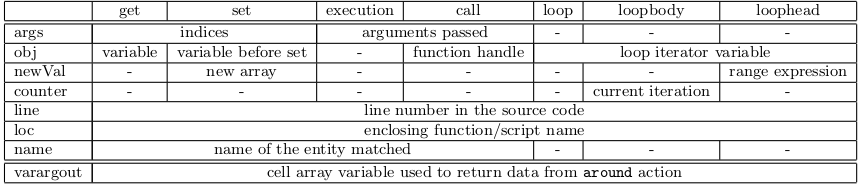
\includegraphics[width=\textwidth]{images/Languages/Matlab_Context.png}
\caption{Context selectors for different join point types.}
\label{tab:Matlab_Context}
\end{table}

\section{Pointcuts}
The pointcuts implemented by AspectMatlab are mentioned earlier when discussing the join point model, therefore I will not discuss them any further but just show an overview in table \ref{tab:Matlab_Patterns}.\\
\begin{table}
\centering
\begin{tabular}{l|l}
\hline
Pointcut & Description\\
\hline
\hline
call & Captures all calls to functions/scripts.\\
execution & Captures the execution of function bodies.\\
get & Captures array accesses.\\
set & Captures array sets.\\
loop & Captures execution of all loops.\\
loophead & Captures the header of the loop.\\
loopbody & Captures the body of the loop.\\
\hline
\end{tabular}
\caption{List of patterns.}
\label{tab:Matlab_Patterns}
\end{table}\\
You can further restrict the scope of matching by using the withing pattern. On the other hand it is also possible to generalize pointcuts by using the wildcards '*' or '..', which can be used to match any function/variable or exactly one argument and one or more variables respectively.\\
\\
Because of the Matlab syntax, where 'foo(1,2)' could either be a call to a function with arguments '1' and '2' or an array indexation, it is possible to create a general notation for calling a function or script and getting or setting a variable. A list of possible matching are given in table \ref{tab:Matlab_PatternExamples}.\\
\begin{table}
\centering
\begin{tabular}{l|l}
\hline
Pointcut & Description\\
\hline
\hline
call(foo) & Matches all calls to foo.\\
call(foo()) & Matches calls to foo with no arguments.\\
call(foo(*)) & Matches calls to foo with exactly one argument.\\
call(foo(..)) & Matches calls to foo with 1 or more arguments.\\
call(foo(*,..)) & Matches calls to foo with 2 or more arguments.\\
call(*(*,..)) & Matches any call with two ore more arguments.\\
\hline
\end{tabular}
\caption{Selective pattern matching.}
\label{tab:Matlab_PatternExamples}
\end{table}\\
You could think that if we were to implement these pointcuts with the new framework we would end up with three subclasses for Pointcut. It is however possible to group them all together into one since there is no clear distinction between a function call and getting a variable. The within would become part of the context provided to the pointcut.

\section{Advice}
AspectMatlab identifies three types of advice being before, around and after. The body of an advice is normal AspectMatlab code as can be seen in listing \ref{lst:Matlab_ExampleCalls}. Since the body of an advice is plain Matlab code this needs no futher explanation.\\
\\
As mentioned before, is it possible to provide context information to the advice. It is also possible to use variables specified within the aspect to communicate between advices or between multiple executions of the same advice. This latter one will cause the most problems as it is currently impossible to do anything like this with the framework. To provide it a work-around where we use static data in the original matlab code can be used. This is however bad coding and breaks the entire concept of aspect oriented programming.

\section{Order}
AspectMatlab introduces a default ordering where the first encountered around advice becomes the outer most one, followed by the rest of the around advices in the order of appearance. After the around advices all the before advices are place in order of occurrence before the actual join point. The some holds for the after advices that are placed right after the join point in the order encountered before the around advices.\\
\\
Since the framework does not provide such a default order, it is required for the AspectMatlab compiler to explicity add such an order to the weaver. This isn't very complicated though, it suffices to remember the last encountered advice of each type (before, around and after) so that when we read a new one we can add create a link between these two advices and mark the stored one as a predecessor of the new one.\\
\\
This solves the order between advices of the same type, what still remains is the order between the different types. There are two different approaches to solve this:
\begin{enumerate}
\item Create a link between the types.
\item Handle the different types one by one in the weaver.
\end{enumerate}
The first approach may sound the best one, but at the same time it does some obsolete work, simply because when weaving we will have to treat every type of advice differently. Which means we could organize them during weaving according to their type.\\
\\
If however it is still preferred to have an order between the different types, which is possible as it might be helpful with certain implementations, this isn't much work to be done.\\
\\
To make all the before advices happen after the last around, we need to store the first encountered before, since we need it at the end to define the last around advice as a predecessor of this first before advice. To make the last after advice happen before the last around advice, since this will be the deepest one and thus the first to be executed after the after, we need to define the last after advice as a predecessor of the last around advice. \\
\\
Because of the order behaviour caused by the around, which makes the order 'reflecting' over the join point, this leads to some confusing ordering and thus it can still not be used that straightforward.

\section{Weaver}
The AspectMatlab compiler (weaver) has been build using extensible toolkits, and aimed for a very clean and modular implementation. It takes a collection of Matlab and AspectMatlab source files as its input and produces a collection of woven Matlab source files. I will not discuss the entire process of how this is done, but a simple overview can be seen in figure \ref{fig:Matlab_Weaver}.\\
\begin{figure}
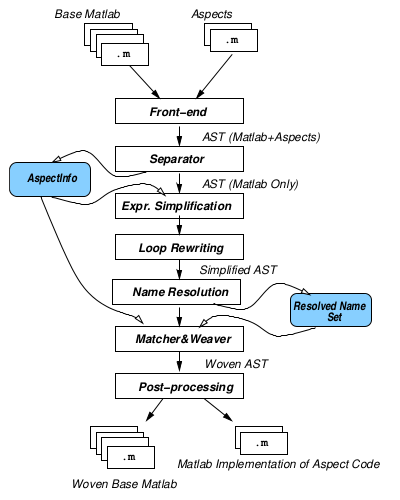
\includegraphics[scale=1]{images/Languages/Matlab_Weaver.png}
\caption{Overal structure of the amc AspectMatlab compiler.}
\label{fig:Matlab_Weaver}
\end{figure}
\\
To be able to call all the advice at the right point, some transformations are required. All expression are disassembled into simple expressions as can be seen in the following example:
\begin{minipage}{0.45\textwidth}
\begin{lstlisting}[caption=Original code.]
z = sum(x) / length(y);
\end{lstlisting}
\end{minipage}\hfill
\begin{minipage}{0.45\textwidth}
\begin{lstlisting}[caption=Resulting code.]
AM_CVar_5 = x;
AM_CVar_6 = sum(AM_CVar_5);
AM_CVar_7 = y;
AM_CVar_8 = length(AM_CVar_7);
z = (AM_CVar_6 / AM_C_Var_8);
\end{lstlisting}
\end{minipage}
\\
It is also important to note that due to Matlab's semantics it is hard to determine at compile time the semantics of a expression. Because they wanted to minimize the amount of run-time checks, they introduced a name resolution analysis which adds extra information to the AST so they can determine the type.\\
\\
Because the current weaver produces a source to source transformation of files, we could implement this the same way using the framework, without requiring any changes to the process.

\section{Examples}
\begin{lstlisting}[caption=An aspect to count all calls made with at least 2 arguments., label=lst:Matlab_ExampleCalls]
aspect myAspect

	properties
		count = 0;
	end

	methods
		function out = getCount(this)
			out = this.count;
		end

		function incCount(this)
			this.count = this.count + 1;
		end
	end

	patterns
		call2args : call(*(*, ..));
		executionMain : execution(histo);
	end

	actions
		actcall : around call2args : (name, args)
			this.incCount();
			disp(['calling', name, 'with parameters(', args , ')']);
			proceed();
		end
		
		actexecution : after executionMain
			count = this.getCount();
			disp(['total calls: ', num2str(count)]);
		end
	end

end
\end{lstlisting}
\begin{lstlisting}[caption=Example of a units aspect., label=Matlab_ExampleUnits]
aspect unit
	patterns
		loopheader : loophead(*);
	end;
	
	actions
		loop : around loopheader : (newVal)
			range = this.annotate(newVal);
			acell = {};
			for i = (range.val)
				acell {length(acell) + 1} = i;
			end
			varagout{1} = struct(this.annotated, true, 'val', acell, 'unit', range.unit);
		end
	end
end
\end{lstlisting}

\section{Difficulties}
The current version of the framework does not cover all features to realize the complete version of AspectMatlab as it is presented. This is a limitation that can easily be fixed by adding those features, as discussed in chapter \ref{chap:FutureWork}. The features that are present in the framework are easy to use for AspectMatlab as the idea behind the elements is similar as those used in Small C.

\chapter{DiSL}
DiSL \citep{marek_disl:_2012} is a domain specific language for bytecode instrumentation. Designing such a language is a complex task as it needs to achieve three conflicting design goals:
\begin{enumerate}
\item high expressiveness
\item high-level programming model
\item high efficiency
\end{enumerate}
Currently there exists low-level languages that meet the first and third goal, but these are based on byte code instrumentation, which makes it hard to develop, maintain and customize tools. Other AOP languages achieve the second goal but do not succeed in exposing important join points, easily provide access to information and mixing bytecode with aspect oriented code.

\section{Join Point Model}
To achieve a high level of expressiveness DiSL has an open join point model, which means that any region of byte code can be a join point.

\section{Base Language Compiler}
DiSL uses Java as its host language and uses annotations to express the functionality required. To parse the base language source code DiSL relies on jBORAT, a lightweight toolkit providing support for instrumentation with complete bytecode coverage.

\section{Aspect Language}
First of all it has to be noted that terminology differs from what is generally used in that way that they use \textit{instrumentation}, \textit{marker} and \textit{snippet} instead of aspect, pointcut and advice. Guards and scopes can be used to restrict the matching of snippets. The difference is that guards are implemented as a class with methods that will be evaluated and should return a boolean value, while scopes limit the execution based on the method signature of the join point.
\\
I've already mentioned some remarks about the aspect language, such as that the code is written as plain Java classes with annotated methods and fields and the open join point Model. Besides having an open join point model, DiSL also allows the user to define his own static and dynamic information which can be used in the snippets. It is also possible to add argument processors which will be used to process arguments.\\
\\
Two examples of DiSL are shown in listing \ref{lst:DiSL_ExampleProfiler} and \ref{lst:DiSL_ExampleSenseo}.

\section{Pointcuts}
To be able to handle the open join point model, DiSL provides an extensible library of markers. These markers are standard Java classes implementing a special interface for join point selection. It has to be noted that in contrary to many other AOP languages these markers are not part of the instrumentation, but are completely implemented on their own.\\
\\
There are two possible ways to implement this with the framework. The first one is doing exactly the same as is done now, but instead of an interface the markers would have to extend the marker pointcut. A problem with this approach is to keep the weaver informed of all these new markers, but that's a problem that can be overcome. Another way would be to create a very general marker pointcut that is able to fit every specified marker such that the parser can create a pointcut with the specified data. This would however cause a lot of problems as the pointcut would be to general making it hard to really suite the desires of the user. What the best solution is is hard to say as the paper does not provide a lot of information about how to specify your own marker.

\section{Advice}
Advice is expressed in the form of code snippets that are inlined, giving the developer fine-grained control over the inserted code. The snippets are written as regular Java static methods and annotations are used to indicate the type, either 'before' or 'after', and other properties such as the marker, guard and scope.\\
\\
Mainstream AOP languages support 'before', 'after' and 'around' advice, but since DiSL is meant for byte code analysis and thus not meant to modify any code, there is no use for the 'around' advice. For that reason DiSL only provides a 'before' and 'after' advice.\\
\\
Thanks to the inlining, snippets are able to efficiently communicate data through local variables defined in the instrumentation, it is also possible to communicate on thread level.\\
\\
A snippet can use both static and dynamic information, which are passed on as an argument, the only possible arguments. Once again it is possible for the user to specify own information by creating a class that implements a certain interface.\\
\\
An advice is pretty simple to implement as it is similar to what we did before. With implementation of the static and dynamic information we face the same problems as with implementing the pointcuts. The framework does not provide a separate mechanism for guards or scope and thus it is required that this information is added to the context of the pointcut.

\section{Order}
Order can be specified for each snippet as a non-negative integer number. The rule is that snippets with a higher order are closer to the join point then snippets with a lower order.\\
\\
The framework does not work with an order value, but instead requires a connection between the advices. This means that the compiler needs to convert these values into an explicit link between advices with consecutive order values.\\
\\
The implicit order of appearance between snippets with the same order value has to be made explicit to the weaver. The parser can do this by making an order while parsing where he states that the previous encountered one must occur before the next encountered.

\section{Weaver}
The DiSL weaver runs on top of jBORAT, which will help us by parsing the classes from the source code. The process of weaving with DiSL goes as follows:
\begin{enumerate}
\item First DiSL parses all the instrumentation classes.
\item When jBorat hands over a class to DiSL an internal representation for snippets, markers, guards, static contexts and argument processes is created
\item Scopes are matched
\item Join point shadows are created and evaluated by guards, and matching snippets are selected
\item Static contexts are used to compute static information
\item Argument processors are evaluated for snippets and matching snippets are selected
\item Everything is woven together
\item Static information and byte code to access dynamic information is added.
\end{enumerate}
This is visually shown in figure \ref{fig:DiSL_Weaver}.\\
\begin{figure}
\centering
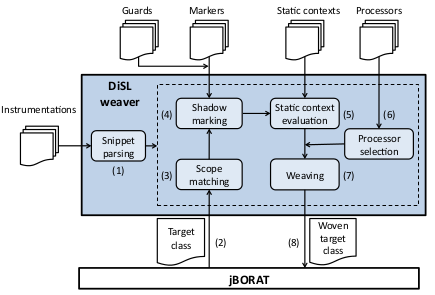
\includegraphics[scale=0.5]{images/Languages/DiSL_Weaver.png}\\
\caption{Overview of DiSL weaving process.}
\label{fig:DiSL_Weaver}
\end{figure}

\section{Examples}
\begin{lstlisting}[language=Java,caption=Aspect for calling context-aware profiling.,label=lst:DiSL_ExampleProfiler]
public class CallingContextBBAnalysis {
	@ThreadLocal
	static CCTNode currentNode;

	@SyntheticLocal
	static CCTNode callerNode;

	@Before(marker = BodyMarker.class, order = 1)
		static void onMethodEntry(MethodStaticContext msc) {
		if ((callerNode = currentNode) == null) {
			callerNode = CCTNode.getRoot();
		}
		currentNode = callerNode.profileCall(msc.thisMethodFullName());
	}

	@After(marker = BodyMarker.class)
	static void onMethodcompletion() {
		currentNode = callerNode;
	}

	@Before(marker = BasicBlockMarker.class, order = 0)
	static void onBasicBlock(BasicBlockStaticContext bbsc) {
		currentNode.profileBB(bbsc.getBBIndex());
	}
}
\end{lstlisting}
\begin{lstlisting}[language=Java,caption=Example for collecting run-time information.,label=lst:DiSL_ExampleSenseo]
public class Senseo {
	@ThreadLocal
	static CCTNode currentNode;
	
	@SyntheticLocal
	static CCTNode callerNode;	
	
	@Before(marker = BodyMarker.class, order = 1)
	static void onMethodEntry(MethodStaticContext msc, ArgumentProcessorContext proc) {
		if ((callerNode = currentNode) == null) {
			callerNode = CCTNode.getRoot();4
		}
			
		currentNode = callerNode.profileCall(msc.thisMethodFullName());
		proc.apply(ReferenceProcessor.class, ProcessorMode.METHOD_ARGS);
	}
	
	@After(marker = BodyMarker.class, order = 2)
	static void onMethodCompletion() {
		currentNode = callerNode;
	}
	
	@AfterReturning(marker = BodyMaker.class, order = 1, guard = MethodReturnsRef.class)
	static void onReturnRef(DynamicContext dc) {
		Object obj = dc.getStackValue(0, Object.class);
		currentNode.profileReturn(obj);
	}
	
	@AfterReturning(marker = ByteCodeMarker.class, order = 0, args = "new,newarray,anewarray,multianewarray")
	static void onAllocation() {
		currentNode.profileAllocation();
	}
	
	@Before(marker = BasicBlockMarker.class, order = 0) {
	static void onBasicBlock(BasicBlockStaticContext bbsc) {
		currentNode.profileBB(bbsc.getBBIndex());
	}
}

@ArgumentProcessor
public class RefferenceProcessor {
	static void objProc(Object obj, ArgumentContext ac) {
		Senseo.currentNode.profileArgument(ac.getPosition(), obj);
	}
}	
\end{lstlisting}


\section{Difficulties}
DiSL is a language completely different from those discussed until now, despite this difference the framework is still able to provide useful functionality proving its value. Besides some minor difficulties, mostly caused by the lack of functionality, there are no big problems if this were to be created with the framework. All the tools that are used to aid in creating this language could also be used to help when working with the framework.

\chapter{Discussion}
\label{chap:Discussion}
As shown by the examples presented, the framework is general enough to be useful in a wide range of languages. The amount of work required to extend the framework depends on the complexity of the target language, and is mostly dominated by the effort required for the weaver. Thanks to the presence of 'helper' methods in the general Weaver, the work that has to be put into the weaver is limited to putting everything together and things as finding matches is done for us.\\
\\
In general we experience that the concept of pointcut and advice as it is captured by the framework provides a good basis to start from and the extensions that are required are very limited. The entire type system however, because it can not be provided by the framework may cause to be problematic. Though if handled well, it is possible to simply re-use the existing type system of the base language eliminating the cost of creating a complete new one.\\
\\
The poincutset which was meant as a way to simplify selecting multiple join point that could not be done by wildcards proves to be very useful, though it can require some new way of thinking since the only supported operator is the logical or. As most other AOP languages support other operators as well, this may seem to be a very limited way to express a set of pointcuts. Upon closer inspection this is often not the case, since for most join points it makes no sense to require that it should happen together with another join point. If we look at the some examples of AspectJ, we note that the '\&' is used with the \textbf{within} keyword. This however is not a join point and is therefore part of the context in the framework.\\
\\
The extended framework and the base language only interact by a compiler that extracts the join points from the source code and by the weaver that adds the advices in the right place. This is however not the only coupling between the base language and the framework, most components that are added to support AOP for the base language will carry some notion of the base language, being it implicitly. Another bit coupling between the framework and the base language is the type system which preferable is the same.\\
\\
Finally we note that modifying the parser for the base language to extract the join points can be quite cumbersome. One way to minimize the required effort would be to use an aspect oriented language and inject the modifications as advice. This way of working is however very limited and can only be done if there is a match between the join point model of the aspect oriented language and the interesting points in the parser. If we would for instance use AspectJ, we are limited to the beginning and end of method executions and calls. If the parser is not sufficiently organized it is impossible to add the code at the right place and the entire approach becomes useless.

\chapter{Future Work}
\label{chap:FutureWork}
The examples discussed here have shown some limitations of the framework. The most important one is the impossibility to communicate between advices. This could be solved by introducing global variables, which would be similar to arguments currently present for advice. The weaving step would have to be extended depending on the way the variables are weaved with the base language source code.\\
\\
Many other AOP languages have an explicit notion of aspect, this is not the case in this framework but could be considered as a valuable addition. Before doing so, it is essential that some questions are answered. Will the aspect only be used to encapsulate global variables, pointcuts and advices or will it be possible to use it like classes in an object oriented language? If that is the case then we gain some valuable features, such as the re-usability of pointcuts. However inheritance would also apply for advice, which means we need a way to select the right advice in case they are overridden. Another problem would be to choose between multiple subaspects, certainly since it may this choice may not be the same for the entire application, but can differ from join point to join point.\\
\\
Another problem with the current framework is the lack of choice between different ways of weaving. Though it is possible to weave the original files and the advice any way you want it is the time of weaving that lacks freedom, and the only real option is using the weaver as a pre-processor. This should be extended to provide more support for run-time weaving, since adding run-time checks isn't always feasible.\\
\\
Another important feature still missing is decent support for debugging, as this is completely left over to the compiler of the target language. This however means that all errors are reported based on the weaved code instead of the original source and aspect files. The easiest way to do this is to encapsulate the final compiler and intercept the errors, by keeping track of the weaved locations we can resolve the errors back to the original locations. This approach can not only be done for 'fixing' the reported errors, but could also be used to handle other tools that work on the weaved code.\\
\\
Currently the framework treats context and arguments in a different way, and is a context more equal to a type as they both define an interface with just an \textbf{isAssignable} method. We could ask ourselves in what way a context would be different from an argument, since in most cases a context variable will have a name and a value, just as an argument.\\
\\
Finally also the weaving process could be optimized to handle quick re-weaving. Currently the weaver starts from the original files every time the process is started. This requires a lot of time for large projects and a lot of weaved code will be the same as the previous, since often only small changes are made at a time. Adding involves adding links between the aspect and source code, which is also required to 'fix' the error messages mentioned earlier.

\chapter{Related Work}
Language Oriented Programming \citep{dmitriev_language_2004} is similar in that way that it provides freedom to the user to create his own DSL, just like the framework allows a user to specify his own Aspect Oriented Language. This is realized by implementing loosely coupled languages which can be combined as requested. Pluggable AOP \citep{kojarski_pluggable_2005} aims to specify aspect oriented languages largely independent of the base language, which would allow combining multiple AOL together.  Though the approach is different as they don't use a framework but a description of the AOL, both aim to get a loose coupling between the AOL and the base language. 

\chapter{Conclusion}
Though the provided functionality of the framework is still somewhat limited, it is able to achieve abstracting the core elements of aspect oriented programming and has been successfully extended to prove its abilities, and its limitations. Despite the limitations of the current framework, it is often already possible to solve the problem in a different way. Yet adding new features and extensions will allow serving an even larger amount of languages and make the framework more user-friendly.

\bibliographystyle{plain}
\bibliography{references}

\end{document}